\documentclass[letterpaper,12pt]{article}
\usepackage[usenames,dvipsnames,svgnames,table]{xcolor}
\usepackage{graphicx}
\usepackage{caption}
\usepackage{subcaption}
\usepackage{tabularx}
\usepackage{amsmath,amssymb}
\usepackage{mathrsfs}
\usepackage{setspace}
\usepackage{enumerate}
\usepackage{todonotes}
\usepackage{listings}
\usepackage{paralist}
\usepackage{natbib}
\usepackage{fullpage}
\usepackage[T1]{fontenc}
\usepackage{booktabs}
\usepackage{pgfplotstable}
\usepackage{makecell}
\usepackage{comment}
\usepackage{soul}
\usepackage{bm}
\usepackage{gensymb}
\usepackage{todonotes}
\usepackage{multirow}

\usepackage[colorlinks=true,
            linkcolor=blue,
            urlcolor=blue,
            citecolor=blue,
            final,
            hypertexnames=true]{hyperref}
\newcommand\myworries[1]{\textcolor{red}{#1}}
\newcommand{\abs}[1]{\ensuremath{ \left|#1\right|}}
\newcommand{\norm}[1]{\ensuremath{ \left|\left|#1\right|\right|}}
\newcommand{\orderof}[1]{\ensuremath{ {\cal O}\left(#1\right)}}
\newcommand{\pdv}[2]{\frac{\partial #1}{\partial #2}}
\newcommand{\grad}[1]{\bv{\nabla} {#1}}
\newcommand{\bv}[1]{{\ensuremath{\boldsymbol{#1}}}}
\newcommand{\bt}[1]{{\ensuremath{\boldsymbol{#1}}}}
\newcommand{\Res}{{\ensuremath{\mathcal R}}}
\newcommand{\Unknowns}{{\ensuremath{\bf{U}}}}
\newcommand{\UnknownsR}{{\ensuremath{\bf{U^R}}}}
\newcommand{\unknown}{{\ensuremath{\bv{u}}}}
\newcommand{\primalsol}{{\ensuremath{\bv{\tilde{u}}}}}
\newcommand{\primalsolh}{{\ensuremath{\bv{\tilde{u}^h}}}}
\newcommand{\adjointsol}{{\ensuremath{\bv{\tilde{z}}}}}
\newcommand{\adjointsolh}{{\ensuremath{\bv{\tilde{z}^h}}}}
\newcommand{\adjointsolH}{{\ensuremath{\bv{\tilde{z}^H}}}}
\newcommand{\Testfuncs}{{\ensuremath{\bf{V}}}}
\newcommand{\testfunc}{{\ensuremath{\bv{v}}}}
\newcommand{\intO}{\ensuremath{\int_\Omega}}
\newcommand{\elem}{\ensuremath{E}}
\newcommand{\qoi}{{\ensuremath{q}}}
\newcommand{\qoih}{\ensuremath{q^h}}
\newcommand{\Qoi}{{\ensuremath{Q}}}
\newcommand{\param}{{\ensuremath{\xi}}}
\newcommand{\params}{{\ensuremath{\bv{\param}}}}
\newcommand{\PDF}{\ensuremath{p}}
\newcommand{\Params}{{\ensuremath{\bf{\Xi}}}}
\newcommand{\ParamsR}{{\ensuremath{\bf{\Xi^R}}}}
\newcommand{\Reals}{{\ensuremath{\mathbb{R}}}}
\newcommand{\sa}{\nu_{\mathrm{sa}}}
\newcommand{\pp}[2]{\frac{\partial #1}{\partial #2}}

%
\newcommand{\uveci}{{\bm{\hat{\textnormal{\bfseries\i}}}}}
\newcommand{\uvecj}{{\bm{\hat{\textnormal{\bfseries\j}}}}}
\newcommand{\uveck}{{\bm{\hat{\textnormal{\bfseries\k}}}}}


\author{Nicholas Malaya}

\begin{document}

%%%%%%%%%%%%%%%%%%%%%%%%%%%%%%%%%%%%%%%%%
% University Assignment Title Page 
% LaTeX Template
% Version 1.0 (27/12/12)
%
% This template has been downloaded from:
% http://www.LaTeXTemplates.com
%
% Original author:
% WikiBooks (http://en.wikibooks.org/wiki/LaTeX/Title_Creation)
%
% License:
% CC BY-NC-SA 3.0 (http://creativecommons.org/licenses/by-nc-sa/3.0/)
% 
% Instructions for using this template:
% This title page is capable of being compiled as is. This is not useful for 
% including it in another document. To do this, you have two options: 
%
% 1) Copy/paste everything between \begin{document} and \end{document} 
% starting at \begin{titlepage} and paste this into another LaTeX file where you 
% want your title page.
% OR
% 2) Remove everything outside the \begin{titlepage} and \end{titlepage} and 
% move this file to the same directory as the LaTeX file you wish to add it to. 
% Then add \input{./title_page_1.tex} to your LaTeX file where you want your
% title page.
%
%%%%%%%%%%%%%%%%%%%%%%%%%%%%%%%%%%%%%%%%%

%----------------------------------------------------------------------------------------
%	PACKAGES AND OTHER DOCUMENT CONFIGURATIONS
%----------------------------------------------------------------------------------------

%\documentclass[12pt]{article}

%\begin{document}

\begin{titlepage}

\newcommand{\HRule}{\rule{\linewidth}{0.5mm}} % Defines a new command for the horizontal lines, change thickness here

\center % Center everything on the page
 
%----------------------------------------------------------------------------------------
%	HEADING SECTIONS
%----------------------------------------------------------------------------------------

\textsc{\LARGE Doctoral Dissertation Proposal}\\[1.0cm] % Name of your university/college

%----------------------------------------------------------------------------------------
%	TITLE SECTION
%----------------------------------------------------------------------------------------

\HRule \\[0.4cm]
{ \Large \bfseries Numerical Simulation of Synthetic, Buoyancy-Induced Columnar Vortices}\\[0.4cm] % Title of your document
\HRule \\[1.5cm]
\textsc{\Large Nicholas Malaya}\\[0.5cm] % Major heading such as course name
\textsc{\large Department of Mechanical Engineering}\\[1.0cm] % Minor heading such as course title
 
%----------------------------------------------------------------------------------------
%	AUTHOR SECTION
%----------------------------------------------------------------------------------------

\begin{minipage}{0.5\textwidth}
\begin{flushleft} \large
{}%{\Huge Nicholas Malaya} \\
%{\normalsize Department of Mechanical Engineering} 
\end{flushleft}
\end{minipage}
~
\begin{minipage}{0.45\textwidth}
\begin{flushright} \large
\emph{Committee:} \\
 \vspace{5mm}
{\Large Dr. Robert D. Moser} \\
{\normalsize \textsl{Advisor}} \\
{\normalsize Department of Mechanical Engineering and Institute for Computational Engineering and Science} \\
 \vspace{5mm}
{\Large Dr. David Bogard} \\
{\normalsize Department of Mechanical Engineering} \\
 \vspace{5mm}
{\Large Dr. Ofodike A. Ezekoye} \\
{\normalsize Department of Mechanical Engineering} \\
 \vspace{5mm}
{\Large Dr. Todd A. Oliver} \\
{\normalsize Institute for Computational Engineering and Science} \\
 \vspace{5mm}
{\Large Dr. Venkat Raman} \\
{\normalsize Department of Aerospace Engineering and Engineering Mechanics} \\
\end{flushright}
\end{minipage}\\[4cm]

%----------------------------------------------------------------------------------------
%	DATE SECTION
%----------------------------------------------------------------------------------------

%{\large \today}\\[3cm] % Date, change the \today to a set date if you want to be precise

%----------------------------------------------------------------------------------------
%	LOGO SECTION
%----------------------------------------------------------------------------------------

%\includegraphics{Logo}\\[1cm] % Include a department/university logo - this will require the graphicx package
 
%----------------------------------------------------------------------------------------

\vfill % Fill the rest of the page with whitespace

\end{titlepage}
%\end{document}


\newpage
\begin{abstract}
\doublespacing

Much of the solar energy incident on the Earth's surface is absorbed
into the ground, which in turn heats the air layer above the surface.
This buoyant air layer contains considerable gravitational potential
energy. The energy can drive the formation of columnar vortices
 (``Dust-Devils'') which  
arise naturally in the atmosphere. A new energy harvesting approach
 makes use of this phenomenon by creating and anchoring the vortices
 artificially and extracting energy from them. In this research
 proposal, we explore the  characteristics of these vorticies through
 numerical  simulation. Computational models of the turning vane system
 which generates the vortex and the turbine used to extract energy
 have been developed. 
 The formulation of these models and their validation
 against available experimental measurements will be discussed, as will
 the details of the columnar vortex structure and its interaction with
 the turbine. In addition, the computational models are being used to
 optimize the turning vane configuration and the turbine characteristics
 to maximize the power extraction, in order to assess the technological
 feasibility of the project. 
 %This optimization and to characterize the effects of
 %environmental conditions such as cross winds and
 %topography. 
 Preliminary results from these studies will also 
 be presented. 
\end{abstract}



\newpage
\tableofcontents
\newpage
%\singlespacing
\onehalfspacing
%\doublespacing
\section{Introduction / Executive Summary}

Renewable energy is critical to our environmental, economic, and
national security. Global demand for energy is projected to rise 56\% by
2040\cite{energy-outlook}, as is our national reliance on fossil
fuel-based power plants for the bulk of our electricity generation. 
There is a critical need for safe, clean, and
cost-effective alternatives to coal, such as wind, solar, hydroelectric,
and geothermal power. These technologies would reduce carbon dioxide
emissions and help position the U.S. as a leader in the global renewable
energy industry. 
% \cite{arpa-e}
% proposal
%
This proposal details a research plan to perform a numerical
investigation and design optimization of a novel renewable energy concept. 

Much of the solar energy incident on the Earth's surface is absorbed
into the ground, which in turn heats the air layer above the surface.
This buoyant air layer contains considerable gravitational potential
energy. 
With nearly one-third of global land mass covered by deserts, there are huge
untapped regions for capturing solar heat (about 200 W/$\text{m}^2$
averaged over a 24-hour day, and up to 1000 W/$\text{m}^2$
peak)\cite{Hoyt197827}. The available power is competitive in magnitude
with worldwide power generation from fossil sources. If a technology
could effectively extract this energy, it would result in a low-cost,
scalable approach to electrical power generation that could create a new
class of renewable energy ideally suited for arid regions.  

How then, is one to efficiently extract this gravitational potential
energy and convert it into usable work? We turn to Nature to provide a 
guide, with the observation that objects already
exist that provide precisely this mechanism. Namely, the phenomena is
that of a naturally occurring ``dust devil'' 
%
% are we certain this is baroclinic? montegomery might argue it is not.
% update: I think montgomery is wrong here, or at best nitty.  
% BAROCLINIC: essentially just that temp fronts exist
%
% update: oops, bob agrees! killing it
%with baroclinic generation of vorticity in a
characterized by a vertically stratified, ground-heated air layer
producing a coherent columnar vortex. These ``dust devil''s are
ubiquitous, naturally appearing in regions as diverse as Arizona,
Siberia, over water, or even
Mars\cite{Sinclair1969,ROG:ROG1635,JGRE:JGRE1660}.  
 % arizona, indiana, oregon, yukon, colorado
They are observed to occur over a wide range of length scales (1 - 30
meters) with large variations in velocities (1 to over 40
m/s)\cite{Sinclair1969}. 

The basic idea behind the proposed energy harvesting approach is to convert the 
potential energy in this buoyant air layer to kinetic energy in an
anchored vortex, and to use that kinetic energy to drive a
vertical-axis turbine coupled with an electric generator  to
produce electrical power. 
The Solar-Driven Vortex (SoV) phenomena has been demonstrated in
an experimental setup by our partners at Georgia Tech. However, to 
move beyond proof-of-concept, Computational Fluid 
Dynamics (CFD) is needed to simulate the SoV. Such simulations will
provide fundamental insight into the 
driving dynamics of the system, generate high resolution data that is 
experimentally inaccessible that can be used to rapidly optimize the
geometry and configuration of the SoV apparatus. 

%This is a considerable effort. 

%
% TODO: add table of 'state of the art' or novel work performed
%

The objective of this project is to assess the technological feasibility of 
using synthetic columnar vortices to generate usable energy. 
This proposal begins in section \ref{sec:physics} with a discussion of the 
naturally occurring phenomenon, the presently understood dynamics of
dust-devils and similar columnar vortices, and the implications for systems
designed to generate their synthetic counterparts. 
In section \ref{sec:mathmodel}, we outline a mathematical model of
the entire system, and in section \ref{sec:software}, we discuss the
algorithms and software implementation used to simulate the
system. Section \ref{sec:validation} discusses the 
validation of these results against existing experimental data and high
fidelity simulations. Section \ref{sec:results} details the preliminary
predictions of system performance in the field, as well as detailing the 
several examples of a numerical optimization of the apparatus. Finally, with the 
preceding sections outlining the present simulation capabilities, 
section \ref{sec:proposed_work} proposes a course of investigation
designed to broadly probe the design space and provide a
definitive assessment of the technological feasibility of the entire 
synthetic columnar vortex concept. 

%details a short validation
%study performed by comparing between the available experimental
%measurements and the simulations results. 

%For these simulations to be generally useful, they must first
%be validated against existing experimental data and high fidelity
%simulations. These models will then explore regimes and scales where no
%experimental measurements presently exist. 
%Characterizing the
%uncertainty of predictions resulting from extrapolation is a critical
%component in enabling reliable assessments of field performance of the
%SoV, as it will guide the commercialization strategy of the product. 


\newpage
\section{Physics of Dust-Devils}

\begin{itemize}
\item phenomenological description
\item regions/frequency of occurance
\item review of sinclair and other pertinent literature
\item known physics of dust devils and other cyclonic structures
\item scaling discussion as estimate of energy
\item Dust-Devil Generation Concept
\item Motivation of computational modeling
\end{itemize}

In order to motivate how best to \textit{engineer} a synthetic
dust-devil, we first address what is known about the naturally occuring
phenomena. We therefore begin this section with a qualitative discussion
of dust-devils, followed by a review of the known physics and pertinent 
literature review. 

Our aim is to simulate the formation of synthetic dust devils in the
field. This requires a model of the ambient conditions for a
representative case, such as Arizona, where experimental data is
available from test have been performed. Furthermore, for this to be
more generally useful in the prediction of flows in a variety of
conditions, we need a model generally applicable to any flow near the
surface of the earth.  
%
% good place to ref jacobson2005fundamentals
%
This document details an analysis of surface fluid mechanics, and
develops a theory of turbulence in a thermally stratified medium. As we
are utilizing a RANS model with spatially variable diffusivity, we are
particularly interested formulating a model for these quantities. 

We are interested in the operation of the apparatus during the day. 
At these times, the atmospheric surface layer has the following character. 
Incident radiation from the sun largely does not interact with the
air, which is nearly transparent. Instead, this radiation is absorbed by
the ground, which causes a temperature rise. This results in a thermal
gradient between the hot ground and the cooler air. The warm ground
conducts heat to the air, causing an expansion and lowering the density
of the air. This reduced density air near the surface is driven upwards
by the force of buoyancy.  

For sufficiently large temperature gradients, these motions are
unstable, and as the warm air is driven upwards the flow will transition
to turbulence. 

OLDER:
\begin{itemize}
\item Qualitative discussion of Sinclair and physics of regime
\item estimates of rayleight number?
\item phenomenological 
\item draw regions
\item eyewall
\end{itemize}


\newpage
\section{Mathematical Modeling}
\label{sec:mathmodel}

% \begin{itemize}
% \item \st{unstable stratified boundary layers (raleigh number estimate)}
% \item \st{justify incompressible N-S}
% \item \st{justification of far-field eddy-viscosity model (M-O)}
% \item modeling eddy-viscosity in device 
% \item vane and turbine representation via penalty function // immersed boundary method
% \item cone representation
% \end{itemize}

%remember that \st{} is strikethrough
%
% should this all be math modeling?
%

The aim of the proposed work is to simulate the formation of synthetic
dust devils in the field. This requires a model of the ambient
conditions for a representative case, such as Arizona, where
experimental data is available from test that have been
performed. Furthermore, for this to be more generally useful in the
prediction of flows in a variety of conditions, we need a model generally
applicable to any flow near the surface of the earth.  

This section details an analysis of surface fluid mechanics, and
develops a mathematical model for turbulence in a thermally stratified
medium. We seek to emulate the operation of the apparatus during the day, 
when dust devils are observed to form readily. 
At these times, the atmospheric surface layer has the following character. 
Incident radiation from the sun does not significantly interact with the
air, which is nearly transparent. Instead, this radiation is absorbed by
the ground, which causes it's temperature to rise. This results in a thermal
gradient between the hot ground and the cooler air. The warm ground
conducts heat to the air, causing expansion and lowering the density
of the air. This reduced density air near the surface is driven upwards
by the force of buoyancy.  

For sufficiently large temperature gradients, these motions are
unstable, and as the warm air is driven upwards the flow will transition
to turbulence. For the typical use case we consider, namely Arizona in
summer, the temperature difference can be in excess of 30 Kelvin. 
Rayleigh numbers associated with temperature gradients of this magnitude
are between $10^{9} - 10^{11}$, and therefore meet the criterion
for transition to a turbulent regime. The flow is that of an unstably
stratified fluid.  

This section begins by describing the governing equations of the system
of interest. It then proceeds to the development of a viscosity model
used to resolve the large scale features of the solution. Next, models
used to represent the vanes and turbine, as well as the separation of
fluid off of these modeled surfaces, are introduced.  Finally, the
models for the computational domain extent and the boundary conditions
are discussed. 

Note that a complete mathematical specification of all the model
parameters introduced in this section are provided in a table in
appendix \ref{app:model_param}.

\subsection{Equations of Fluid Motion}
\label{sub_sec:ns_en}
%
% do I need to justify this more? These are pretty critical, after all
%

The equations describing fluid flow with natural convection are,
\begin{align}
  \frac{\partial u}{\partial t} + u \cdot \nabla u =& \,
  -\frac{1}{\rho}\nabla P + \nu \nabla^2 u - g \frac{T'}{T_0}\\
  \nabla \cdot u =& \, 0 \\
  \rho c_p \frac{\partial T}{\partial t} + u \cdot \nabla T =& \, \nabla \cdot ( k \nabla T).
\end{align} 

The makes the assumptions that the temperature variation is small in
comparison to the mean temperature of the region. These are the
incompressible Navier-Stokes equations with Boussinesq representation of
buoyancy coupled with the heat equation.  
%
% in full document be sure to mention that neglecting coriolis is legit
% below 50ms
%
%
As discussed above, we anticipate our flow to be
turbulent. Turbulence significantly alters the character of the flow,
and necessitates either resolving the resulting small scales or
providing a model that emulates their impact. In this case, we use a
Reynolds Averaged Navier-Stokes (RANS) formulation, where we 
permit the viscosity and thermal conductivities to vary in space, and
decompose the flow into constant laminar and varying turbulent and vane
components,  

% \begin{eqnarray*}
%  \nu =& \nu_{l} + \nu_{T}(z) + \nu_{V}(r,z) \\
%  K =& K_{l} + K_{T}(z) + K_{V}(r,z)
% \end{eqnarray*}

\begin{eqnarray*}
 \nu =& \nu_{l} + \nu_{T}(z) + \nu_{V}(r,z) \\
 K =& K_{l} + K_{T}(z) + K_{V}(r,z).
\end{eqnarray*}

This is an effective eddy viscosity model, and the subsequent two
sections will elaborate on the spatial dependence and character of
$\nu_T$, $K_T$, $\nu_C$ and $K_C$. $\nu_l$ and $K_l$ are the laminar,
base diffusivities and do not vary in space. 

\subsection{Viscosity Model}

We use the celebrated similarity model of Monin and
Obukhov\cite{monin2007statistical,monin1954basic} as a guide to the
present development, which we outline below. Their formulation is an
extension of the mixing-length model of Prandtl, where the concepts of
gradient diffusion and mixing length were generalized to thermally
stratified flow.   

%
% justify prandtl assumption here
%

Monin and Obukhov argued that under temporally steady, horizontally
homogeneous conditions, the dynamics of any mean turbulent quantity
($\bar f$) in a thermally stratified medium which depends only on,  

\begin{equation}
\bar f = f(z,\frac{g}{T_0},\rho_0,\nu_l,K_l,u^*,q).
\end{equation}
Aside from near the surface, the laminar diffusivities $\nu_l$ and $K_l$ will be
 small compared to their turbulent counter-parts, $\nu_T$ and $K_T$, and
 are therefore negligible. 
The remaining five parameters are: the distance from the ground, z; the
buoyancy coefficient, $\frac{g}{T_0}$; the density of the fluid,
$\rho_0$; a velocity scale, $u^*$; and the heat flux from the ground,
$q$. 
% Likewise, if we define $z-z_0$ as an ``effective roughness
% height'' or displacement distance, we can reasonably neglect $z_0$ from these
% considerations. While the roughness height can be large (for instance in
% a cornfield, where the roughness height could reasonably be several
% meters), for the present study the expectation is that this roughness
% height will be on the order of centimeters\cite{oke1987boundary}, and
% therefore negligible.  
%
% add refence to dynamical and physical meteorology 
% 
These quantities depend on four dimensions: length, time, temperature
and mass. Dimensional analysis implies that this mean turbulent quantity
($\bar f$) should then only be a function of a single dimensionless
group\cite{munson2012fundamentals}. This is chosen to be,
\begin{equation}
 \xi = \frac{z}{L_{M-O}}.
\end{equation}
$L_{M-O}$ is the famous, ``Monin-Obukhov'' length,
\begin{equation}
 L_{M-O} = -\frac{{u^*}^3}{\kappa \frac{g}{T_0} \frac{q}{c_p \rho_0}}
\end{equation}
where $\kappa$ is the (dimensionless) Von-Karman constant. 
The physical meaning of $L_{M-O}$, the Monin-Obukhov length, bears some discussion. 
The numerator is proportional to the kinetic energy generated by the ambient 
shear of the fluid. The denominator is the buoyant production of kinetic energy. 
As a result, this length scale can be interpreted as the physical location where the
production of buoyant kinetic energy is approximately equal to the energy generated 
by wind shear. When the magnitude of $L_{M-O}$ is large, the flow is dominated
by shear effects, and the impact of buoyancy is small. Conversely, a small 
magnitude of $L_{M-O}$ implies that buoyant effects largely dominate the kinetic energy production.

%The mean quantity $\bar f$ has a
%functional representation to the effect,
Then appropriately normalized mean turbulent quantities should be
functions of only the non-dimensional group 
\begin{equation}
 \frac{\bar f}{f_{MO}} = \phi(\xi)
\end{equation}
with $f_{MO}$ a normalizing constant with units of $\bar f$, and $\phi$ is a
function only of $\xi$. We are interested in the case where $\xi<0$, which
corresponds to heat flux from the ground into the air.
For instance, the mean velocity field would have
scaling, $\frac{u^*}{\kappa}$ and the temperature fields would be scaled
as $T^* = \frac{1}{\kappa u^*} \frac{q}{c_p \rho_0}$. In this way, the
mean velocity and temperature fields would have the form, 
\begin{eqnarray}
\bar u(z) = \frac{u^*}{\kappa} \phi_u(\frac{z}{L_{M-O}}) \\
\bar T(z) = T^* \phi_T(\frac{z}{L_{M-O}}).
\end{eqnarray}
As a result, the vertical gradients of the velocity and temperature are
necessarily, 
\begin{eqnarray}
\frac{\partial \bar u(z)}{\partial z} = \frac{u^*}{\kappa L_{M-O}}
 \varphi_u(\frac{z}{L_{M-O}}) \label{eq:uz} \\ 
\frac{\partial \bar T(z)}{\partial z} = \frac{T^*}{L_{M-O}}
 \varphi_T(\frac{z}{L_{M-O}}) \label{eq:tz}.
\end{eqnarray}
Notice that $\phi$ and $\varphi$ are different universal functions. Eddy
viscosity is defined as, $u'v' = \nu_T \frac{\partial
u}{\partial z}$\cite{durbin2001statistical}, in which case, using
equation \ref{eq:uz}, it must scale as,  
\begin{equation}
 \nu_T = \frac{{u^*}^2}{\frac{\partial \bar u}{\partial z}} = \frac{u^*
  \kappa L_{M-O}}{\varphi_u(\xi)}.
\end{equation}
While eddy thermal diffusivity (defined as, $q = c_p \rho_0 K_T \frac{\partial T}{\partial
z}$) is, 
\begin{equation}
 K_T = \frac{q/c_p \rho_0}{\frac{\partial \bar T}{\partial z}} = \frac{u^*
  \kappa L_{M-O}}{\varphi_T(\xi)}.
\label{eqn:eddy_kt}
\end{equation}
Note that while we have differentiated between $\varphi_u$ and
$\varphi_T$, for turbulent Prandtl numbers near unity (e.g. $Pr_T
\approx 1$) the functions will be identical. The asymptotic behavior of
the $\varphi_T$ and $\varphi_u$ at 
large and small values of $\xi$ provides guidance on more general character of the
functions. We are interested in the case where $L_{M-O}<0$, which corresponds to 
heat flux from the ground into the air. 
%


The case where $\xi \to -\infty $ implies $\frac{z}{L_{M-O}} \to
-\infty $ and $z>>L_{M-O}$. This is most readily interpreted as the instance
where $u^* \to 0$, e.g. the buoyancy-dominated case with no wind
(free-convection). For this case, the function $\varphi_T$ must hold no
dependence on $u^*$, and will approach a constant value. Scaling
analysis implies that the overall function will not depend on $u^*$ only
when the function $\varphi$ scales to the $-\frac{4}{3}$ power. The
resulting function appears as

\begin{equation}
 K_T = \frac{1}{C_T} \left( \frac{q}{c_p \rho_0} \frac{g}{T_0}
		     \right)^\frac{1}{3} z^{\frac{4}{3}}  \text{ 
for } z \gg L_{M-O}. 
\end{equation}

So long as the Prandtl number remains constant in space, then
% todo: provide discussion as to why this is not an unreasonable expectation
identical arguments as to the asymptotic behaviour at large $\xi$ provide
the analogous result for the eddy viscosity's variation with respect to
distance from the ground,  
\begin{equation}
 \nu_T = \frac{1}{C_{\nu_T}} \left( \frac{q}{c_p \rho_0} \frac{g}{T_0}
			     \right)^\frac{1}{3} z^{\frac{4}{3}}  \text{ 
for } z \gg L_{M-O}. 
\end{equation}

These functions have been found to be broadly applicable and
accurate\cite{Foken2006}, and are easily instantiated in software.

\subsection{Eddy Viscosity in Device}

%However, this is also a more
%difficult regime to model.\todo{poor justification} 
The validation process identified a refinement to the virtual vane
formulation that results in a better representation of the vane
effects in a broader range of flows. 

The thermal and momentum diffusivities are even larger in the
device where the flow across the vanes produces shear and generates
turbulence. The model now include an enhanced turbulent diffusivity in
the vortical plume region to account for the effects of vortex shedding
from the trailing edge of the vanes, which is not inherent in the
virtual vane representation.   

% To successfully accomplish this, source terms
% for production of diffusivity were formulated to properly
% account for the generation of turbulence in the region of the
% vanes. This diffusivity would then convect and diffuse through space. 
% To avoid modeling a temporal and three-dimensionally spatially
% varying field of diffusivities, we have instead calibrated the field
% based on data provided by our partners at Georgia Tech. 

%This calibration
%is detailed in Section \ref{sec:validation}. 
The eddy-viscosity in the region of the vanes and interior is set based
on scaling relations for a turbulent self-similar circular jet, as in 
Pope\cite{pope2000turbulent}
 
\begin{equation}
  \nu_C = U_0 y_{1/2} \bar \nu_C.
  %\nu_C(r) = U_0(r) y_{1/2}(r) \bar \nu_C
\end{equation}

In this equation, $U_0$ is the peak velocity, and $y_{1/2}$ the jet
half-width (taken to be the dust devil half-width).  
% In words, we are scaling the
% calibrated viscosity by the velocity and length scale of the
% apparatus. $\bar \nu_C $ is input, measured from the experimental
% laboratory.  The diffusivity here is essentially a top hat filter, which
% radial values interior to the vanes the nominal calibrated value, and
% those outside the vanes zero, e.g. $\nu_C(r>r_{\text{vane}})=0$. 
The dimensionless constant $\bar \nu_C $ is calibrated based on
experimental data, and is set to zero outside the device. 
The thermal diffusivity inside the device, $K_C$, is then fixed with the 
assumption that the Prandtl number is unity.  

%The thermal and momentum diffusivities are expected to be even larger in the
%device where the flow across the vanes produces shear and generates
%turbulence. Our model for the diffusivities inside the vanes should
%therefore be higher than the ambient regions outside the vanes. 



\subsection{Vane and Turbine Representation}
\label{subsec:vane}
To rapidly prototype general system configurations, the
computations must be able to explore a large space of possible
geometries and settings. This presents a significant meshing and 
computational challenge if the detailed flow around the vanes is to be
computed. In the region near the vanes, where a no-slip boundary
condition is imposed, the flow will necessarily form a thin momentum
boundary layer. Resolving this boundary layer requires high resolutions
immediately adjacent to the walls. Changing the vane location requires
that a new mesh be generated.
This is a significant
challenge, as the development of a new mesh often requires significant
human effort and time. Furthermore, the process is error-prone, 
and would require that each simulation using a new mesh undergo 
detailed solution verification. 


% Your text on the virtual vanes does not provide enough information to
% know exactly what we did. It is needlessly vague, and does not
% adequately connect to the real vane geometry. I propose the following
% more direct and more precise text. Further, the penalty nomenclature
% is inappropriate.

Instead, we have developed a modeling formulation that does not require
explicitly meshing the turning vanes, or any surface. These so-called
"virtual vanes" are implemented as a body force that 
is applied in the annular region that contains the vanes. Vane
geometry is specified by the angle $\phi$ a vane makes with a radial
line as a function of the radial coordinate $r$. A unit normal to vane
surfaces ${\bf n}$ is thus defined as
%
\begin{equation}
 {\bf n}({\bf x}) = \sin \left(\phi(r) \right) \hat{{\bf r}}+ \cos \left(\phi(r) \right) \hat{{\bf \theta}}
\end{equation}
%
where $\hat{{\bf r}}$ and $\hat{{\bf \theta}}$ are unit
vectors in the radial and azimuthal directions respectively.
With this vane-normal vector field specified, a body force ${\bf f_v}$
is defined
that will drive the velocity in the ${\bf n}$ direction toward zero,
effectively turning the flow to be parallel to the vanes. The body
force is defined:
\begin{equation}
 {\bf f}_v= -\frac{1}{\ell_v}|{\bf u}|({\bf u}\cdot{\bf n}){\bf n}
 \label{eqn:body_force}
\end{equation}
with ${\bf u}$ the velocity and $\ell_v$ is a specified length
scale. The length scale $\ell_v$ represents the distance over which the
flow evolves under the influence of the body force before the
velocity in the normal direction is reduced by a factor of $1/{\bf
e}$. In other words, this is the distance over which the
normal component of the velocity decays exponentially.
It is a modeling constant and is specified to be
the same order as the separation distance between neighboring vanes in
the physical vane configuration, since entry lengths in internal flows
scale with the size of the channel.

This virtual vane formulation is similar to the ``actuator disk'' model
commonly used to represent the rotor of a wind turbine \cite{betz}.


\subsection{Solid Surface Representation}
\label{subsec:solid_surface}

This subsection details the model used for rigid, impermiable surfaces
such as the wind break (``cone'') on the top of the facility. As with
the turning vanes, this is accomplished without explicitly meshing the
surface nor imposing  a boundary condition at the surface. This permits
rapid exploration of configurations  with different solid surfaces to
control and manipulate the fluid flow. These solid surfaces are also
represented by a body force region applied where the wall is set to be
located in.  A vector normal to the surface is defined in this region so
that a body force will push  the velocity to zero, resulting in the flow
moving only parallel to the virtual surface. For instance, the outward
facing unit normal for a cylindrical surface is represented as 
\begin{equation}
 {\bf n}({\bf x}) = \hat{{\bf r}}+ \sin \left(\theta\right) \hat{{\bf \theta}}.
\end{equation}
In this equation, $\theta$ is the angle between the spatial location and
radial line. The body force is defined as in equation
\ref{eqn:body_force}; however, the length scale $\ell_v$ is specified to
be identical to the width  of the surface being represented. This is
typically two or three grid points. While the actual surface we are
emulating is thin, the numerical method has difficulty converging for
surfaces smaller than the grid size.  

Forcing designed to mimic a surface
is not unique to this project, and is closely related to (among others)
the ``immersed boundary methods'' used by various other
researchers\cite{doi:10.1146/annurev.fluid.37.061903.175743}. 
This approach is unique in its use of Babuska's penalty treatment of
constraints\cite{1973fempen,ZAMM:ZAMM19880680925} to enforce the
behavior at the boundary. This method was selected because it is easily
imposed in the FEM context, and the method has been explored in detail
in the literature. Typically, the enforcement occurs along a domain
boundary, but in this work it is used in the interior. 

As an example, consider Laplace's 
equation on a domain $\Omega$ with boundary $\partial\Omega$, 
\begin{equation}
 \nabla^2 u = 0. 
\end{equation}
Dirichlet boundary conditions are introduced into the weak form
\begin{equation}
 u|_{\partial \Omega} = g
\end{equation}
which becomes 
\begin{equation}
\int_{\Omega}  - \nabla u \cdot \nabla v \, dx - \frac{1}{\epsilon}
 \int_{\partial \Omega} (u-g) \cdot v \, ds = 0 \quad \forall v \in H^1(\Omega)
\end{equation}
where $v$ is an appropriate test function, $\frac{1}{\epsilon}$ is the
penalty parameter and $H^1(\Omega)$ is the Sobolev space of functions on
$\Omega$. This is the weak form for Laplace's equation with a Robin boundary condition 
\begin{align}
 u = g - \epsilon \, \partial_n u. 
\end{align}
For sufficiently small $\epsilon$, the original Dirichlet boundary
conditions will be satisfied approximately. Clearly, $\epsilon$ has
units of length, and can be interpreted as a ``slip length''. 

%
% In the
% Navier-Stokes solver, this penalty formulation is used to approximately
% impose the no-flow through for impermiable surfaces, such as the
% cone.
%
%
% you will need to motivate and then write down your actual formulation
% including the finite width of the forcing layer
%
% these should be written down mathematically
%

By analogy with the method above, we add a penalty term to the weak
form of the Navier-Stokes momentum equation described in the subsequent
section %\ref{eq:ns_weak} 
that has the form, 
\begin{equation}
P_\epsilon = \int_\Omega ({\bf f_v} \cdot v) \, dx
\end{equation}
where ${\bf f_v}$ is as described in equation \ref{eqn:body_force}. 
As the system is formulated as a variational problem that seeks to
minimize the test function $v$, any velocity that is not aligned with
the vane normal will incur a penalty versus one that does. Note that unlike
some penalty methods, this does not automatically satisfy
continuity. Rather, the velocity field remains divergence free through a
separately enforced constraint.  

\subsection{Separation Model}

In the presence of wind, it was found that there was a significant flow
out through the vanes in the back of the device. This was obviously
inconsistent with the findings of our colleagues in the field, who
observed no outflows out of the back of device. Moreover, this resulted
in large inconsistencies between our predictions and the field results,
almost certainly because of the kinetic and thermal energy that our vane
representation was permitting to leave out the back of the device.  

This exposed a weakness of the turning vane representation outlined
previously. When the flow entered the virtual vane forcing region it was
always turned to align with the vane angle, even when the forcing was in
the opposite direction of the present velocity.
This is in contrast to our physical intuition, where we
expect the flow to continue along an averaged streamline
off the trailing edges of the vanes, instead of turning around. 
The averaged streamline (e.g. the statistically average behavior, not
an instant flow field) will continue past the trailing edge of the vane
due to the separation of the boundary layer off the edge surface. An
image depicting these two cases in shown in figure \ref{fig:sep_model}.  

\begin{figure}[!htb]
  \begin{center}
    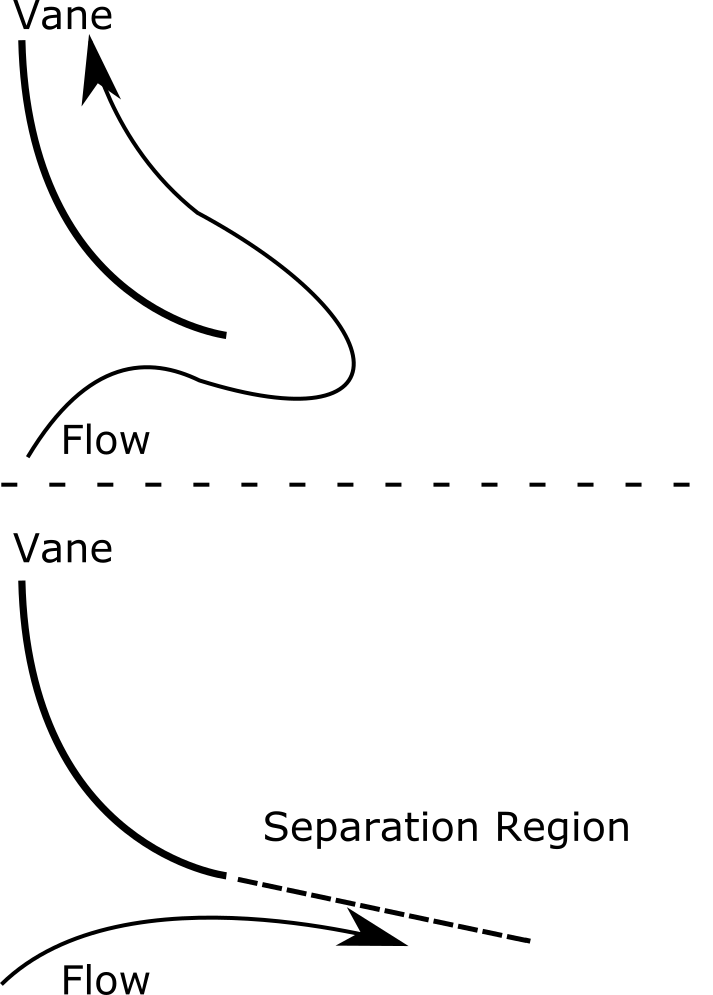
\includegraphics[width = 6 cm]{figs/sep_model}
    \caption{Schematic depicting the separation model that extends past
   the trailing edge of the vanes. In the top case, the flow entering
   the virtual vane region is forced to align with the vane angle despite
   this resulting in a reversal of the flow direction. This is a
   consequence of the forcing function acting on the fluid to ensure the
   velocity vector aligns with the vane. 
   The second case depicts the separation
   model, where the flow under certain conditions is not forced and
   continues to move tangent to the vanes due to 
   the separation of the boundary layer off the trailing edge.} 
    \label{fig:sep_model}
  \end{center}
\end{figure}

Let $\bf n^v$ be the normal vector to the vanes in a horizontal plane,
and $\bf n^r$ the normal vector pointing out of the vane
region\footnote{\normalsize The superscripts ``v'' and ``r'' stand for
vane and radial, respectively.}.  
Then, $\bf t^v$ is the tangential vector to the vanes pointing out of
the vane region and is defined as,
\begin{equation}
 \bf t^v = \left( {\bf n^v_y},{\bf -n_x^v} \right) \text{sign}\left[
	    \left( {\bf n^v_y},{\bf -n_x^v} \right) \cdot {\bf n^r} \right].
\end{equation}


%
% example of an algorithm
%
\begin{center}
 \begin{algorithm}
  \caption{The crude separation model. This model identifies if the flow
  is coming into or out of the vane region, and if the velocity vector
  is in the same direction as the tangent line of the vanes. In the
  algorithm below, $r_0$ is the max radius of vanes, $r_i$ the minimum
  radius of vanes, and $\delta$ is the width of the separation region.}
  \label{alg:sep}
  \begin{algorithmic}[1]
   \If{($r_0 > r > r_i$)} 
   \If{$(r_0 - r) < \delta$ \textbf{or} $((r - r_i) < \delta)$}
   \State $\overrightarrow{n^r} = \overrightarrow{r}/|r|$
   \If{$(r - r_i) < \delta$} 
   \State $\overrightarrow{n^r} = -\overrightarrow{n^r}$
   \EndIf
   \State $\overrightarrow{t^v} = (n_y^v , -n_x^v) \text{ sign
   }((n_y^v,-n_x^v) \cdot \overrightarrow{n^r})$
   \If{$v \cdot t^v > 0$ \textbf{and} $v \cdot n^r < 0 $}
   \State Special Forcing
   \Else
   \State Normal Forcing
   \EndIf
   \Else
   \State Normal Forcing
   \EndIf
   \EndIf
  \end{algorithmic}
 \end{algorithm}
\end{center}
%

The forcing is modified when the velocity vector of the local flow, $\bf
u$ is pointing in to the forcing region: ${\bf u} \cdot {\bf n^r} < 0$, and
when the velocity vector is in the same direction as the tangent line to
the vanes: ${\bf u} \cdot {\bf t^v} > 0 $. In these instances, the
forcing acts as if there was a rigid surface past the vane edge, and
gives the appearance of a special ``no-penetration'' condition for the
velocity for these cases. The pseudo-code for this procedure is shown in
algorithm~\ref{alg:sep}.

The addition of this simple separation model significantly reduced the
flow that penetrated the back of the vanes, and produces results
consistent with the observations provided by our experimental
colleagues.  

\subsection{Effect of Surface Roughness}

%%
%% this does not describe the phenomena being modeled or the precise
%% model -- rewrite
%%
%%
%% this does not say enough about the surface roughness
%% motivate that and explain how it is used, than show your estimate 
%% to argue it is small
%%

Surface roughness effects have been shown to play a role in the
formation of dust-devils and related atmospheric
phenomena\cite{oke1987boundary}. For the flat and sandy regions we are
simulating, the impact is expected to be a small thermal ``kick-up''
versus an entirely smooth surface. This is modeled as a volumetric 
forcing over a narrow height over the surface, 
\begin{equation}
 F^{'''}_{z_0} = \frac{1}{2}\rho V_z^2/z_{0}, 
\end{equation}
and $z_{0}$ is the roughness height. We ensure that the energy
introduced into flow is small fraction of total flow energy by comparing
this with the energy flux through the top of the vanes. The total energy
added is measured as,  
\begin{equation}
 E_{\text{injected}} = \int_0^{2\pi} \int_0^R \int_0^{z_0} F^{'''}_{z_0} dz dr d\theta. 
\end{equation}
R is the outer diameter of the vanes. 
The value of $E_{\text{injected}}$ is typically a few percent of the
total energy kinetic energy flux measured through the top of the
vanes.

%This general forcing provides additional capabilities including the
%ability to investigate engineering greater surface roughness or
%structures that could provide greater ``kick-up'' of the thin thermal
%layer near the surface into the flowing regime. It can also support more
%general turning configurations than the virtual vanes outlined above. 

\subsection{Simulation Geometry and Boundary Conditions}
\label{sec:bc}

This project has two principle modeling regimes. One for the
``thermal-only'' simulations,  which is a domain with no ambient
velocities and an imposed temperature on the ground.  The other
simulation regime of interest is where ambient winds also contribute
(``wind'' cases). We now describe these two scenarios in terms of the
choice of domain extent as well as the boundary conditions. 

\textbf{Computational Domain} 

All simulations are performed in a cuboid domain, with six
faces.  The domain is defined as $\Omega \subset \mathbb{R}^3$. 
The domain extents are scaled by the system diameter, D created by the outer vane radius. 
The extents are defined in terms of $\{L_x,L_y,L_z\}$ indicating the 
streamwise, spanwise and vertical directions, respectively. 
For the thermal-only, which is identical in $L_x$ and $L_y$, the system extents
($L_x/D$,($L_y/D$) are chosen to be 3. The height ($L_z/D$) is three
times the system diameter, which is typically nearly equal to the height
of the vanes. This defines the domain $\Omega$, 
for instance the thermal-only domain is 
$\Omega_T = \left[-L_x,L_x \right] \times \left[-L_y,L_y \right] \times \left[0,L_z \right]$. 

For the wind cases, the streamwise extent is no longer equal to
the spanwise length, $L_y$. In these cases, the domain length extends
two diameters in front of the vanes and three behind. The
spanwise direction is symmetric extends two diameters in each direction 
from the center ($L_y/D = 2$). The height is identical to the thermal-only case, at
three system diameters ($L_z/D = 3$). Thus, the wind domain is 
$\Omega_W = \left[-2D,3D \right] \times \left[-L_y,L_y \right] \times \left[0,L_z \right]$. 

The boundary the the thermal only case is decomposed as,
$\partial \Omega_T = \Gamma_G \bigcup \Gamma_T \bigcup \Gamma_P $. 
$\Gamma_G$ corresponds to the boundary along the ``Ground'', $\Gamma_T$ the ``Top'' boundary,
and $\Gamma_P$ the four periodic ``Sides''. A 3d diagram labeling these boundaries is shown in
Figure~\ref{fig:thermal3d}. For this case study (no mean wind), 
periodic boundary conditions are used on the four sides , and a modified
``inflow-outflow'' Neumann condition\cite{gunzburger1989finite} on the
top boundary, On the ground, a ``no-slip'' velocity boundary condition is
imposed on the velocity field, and a Dirichlet condition uniformly fixes
the temperature of the surface. 
Each of the $\Gamma$ boundary terms are defined in the subsequent labeled paragraphs.  
Note that a finite thickness ``Sponge Layer'' is labelled on the figure along 
the top boundary and is defined in a section below.

\begin{figure}[!htb]
  \begin{center}
    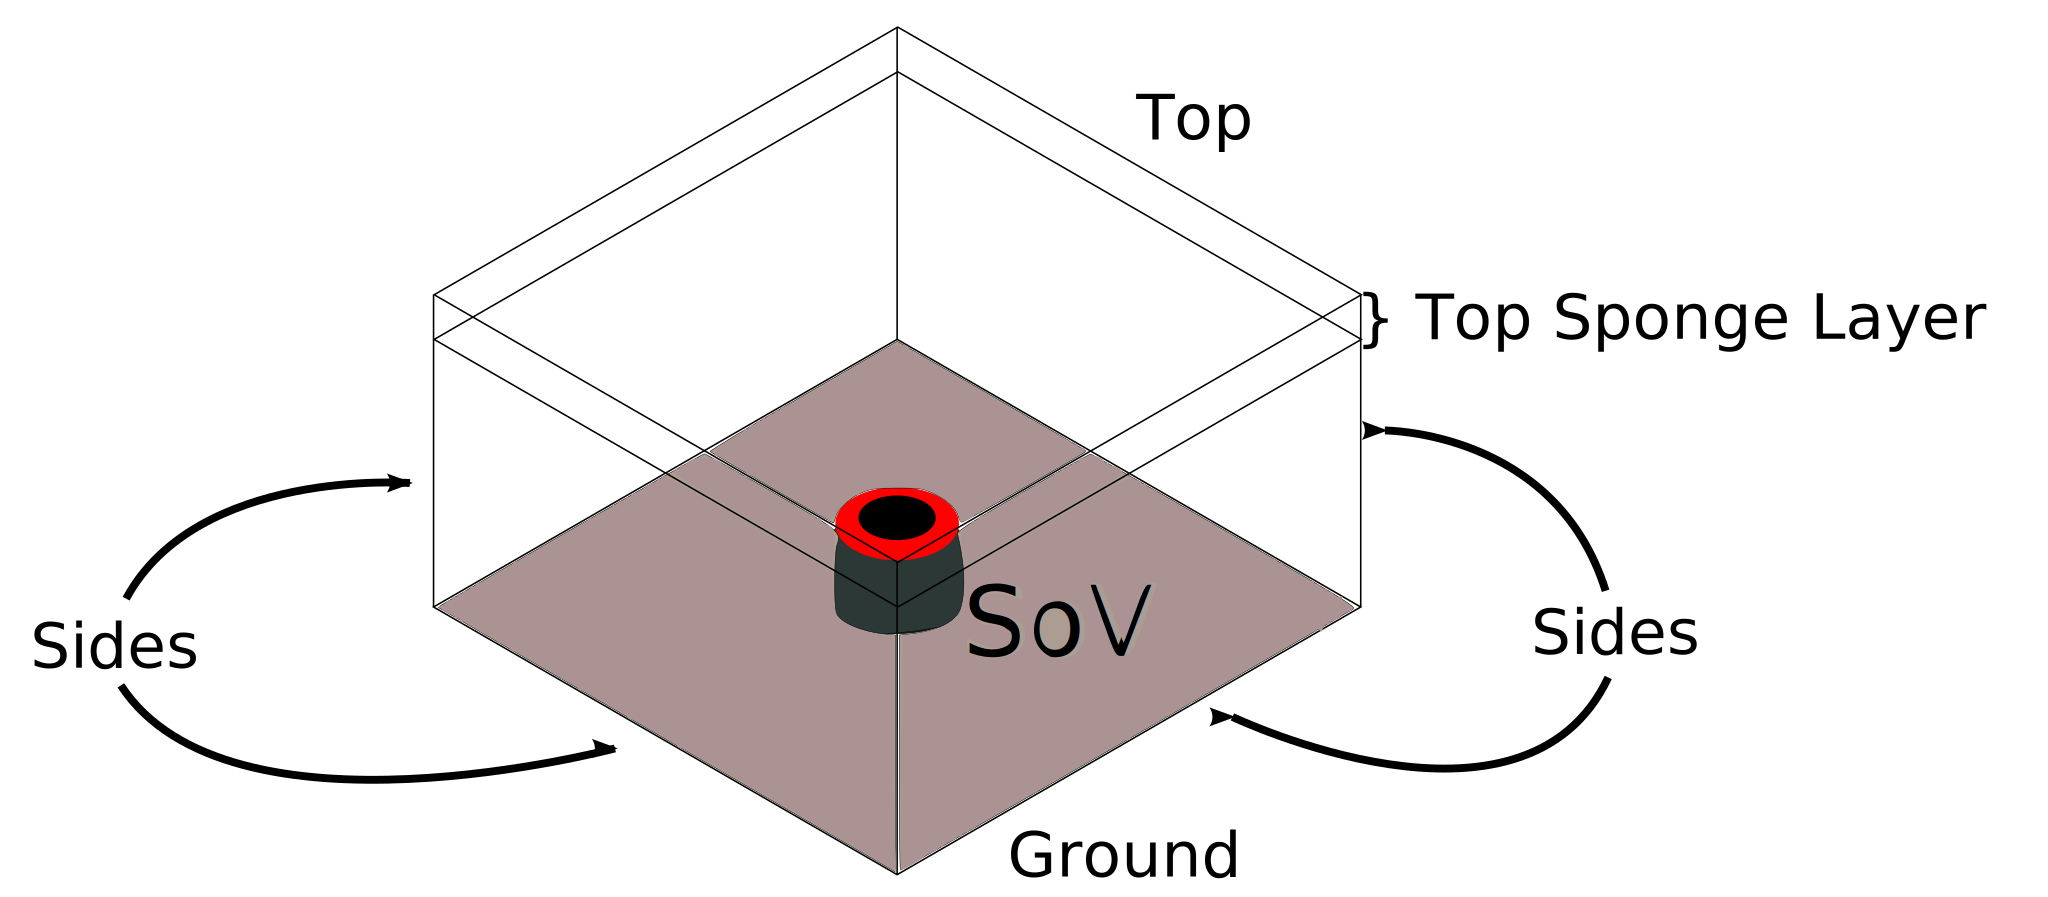
\includegraphics[width = 14 cm]{figs/thermal_only_3d}
    \caption{Domain for the thermal-only
   scenario. The diagram scale is representative of typical cases. Note
   the SoV apparatus in the center, which provides perspective on the
   extent of the domain with respect to the turning vane diameter. The
   ground, sides and top boundaries are labeled with the discussion the
   precise boundary conditions on each provided in
   section~\ref{sec:bc}. Notice also the finite thickness, high
   viscosity ``sponge layer'' at the top of the domain.} 
    \label{fig:thermal3d}
  \end{center}
\end{figure}

The boundary for the wind cases is decomposed as,
$\partial \Omega_W = \Gamma_G \bigcup \Gamma_T \bigcup \Gamma_O \bigcup \Gamma_I \bigcup \Gamma_S $. 
Where $\Gamma_G$ corresponds to the boundary along the ``Ground'', $\Gamma_T$ the ``Top'' boundary, 
$\Gamma_S$ the two ``Sides'', $\Gamma_I$ the inflow boundary, and $\Gamma_O$ the ``Outflow'' 
boundary.
A 3d representation of the ``wind'' simulation is diagrammed in
Figure~\ref{fig:wind3d} and labels the boundaries. 
For this particular study (a heated ground with 
an ambient wind), the wind case has a proscribed inlet boundary layer along the 
upstream streamwise face ($\Gamma_I$)
for both the temperature profile as well as the velocity. The ``Ground''
boundary is identical to the thermal-only case. The ``Sides'', ``Outflow'' and
``Top'' are all set to modified Neumann boundary conditions. 
Note that ``Sponge Layers'' are used on both the back boundary as well as the top.

\begin{figure}[!htb]
  \begin{center}
   %\includegraphics[width = 14 cm]{figs/wind_3d}
   \includegraphics[width = 14 cm]{figs/wind_3d}
    \caption{Domain for the wind and thermal scenario. The diagram scale
   is representative of typical cases. Note the SoV apparatus which
   provides perspective on the extent of the domain with respect to the
   turning vane diameter. The ground, sides, inflow, back and top
   boundaries are labeled with the discussion the precise boundary
   conditions on each provided in section~\ref{sec:bc}. Notice also the
   finite thickness, high viscosity ``sponge layer'' at the top and back
   of the domain.}   
    \label{fig:wind3d}
  \end{center}
\end{figure}

\textbf{Ground Boundary Conditions, $\Gamma_G$} 

For both the wind and thermal-only cases the ground has a fixed
temperature and no-slip velocity boundary conditions. This boundary 
($\Gamma_G$) is modeled with a Dirichlet boundary condition such that, 
\begin{align}
 \overrightarrow{u} &= 0 \quad \text{ on } \Gamma_G \\
 T &= T_g
\end{align}. 
Where $\Gamma_G = \{(x,y,0) \subset \partial \Omega \} $. 

%
% http://fenicsproject.org/documentation/dolfin/dev/python/demo/documented/periodic/python/documentation.html 
%
%
\textbf{Periodic Boundary Conditions, $\Gamma_P$} 

A periodic boundary condition is used in the thermal only cases, 
along the streamwise and spanwise boundary faces 
(denoted $\Gamma_{P,x}$ and $\Gamma_{P,y}$, respectively). In these cases the state variables 
are made to agree with the value at the opposite face, for instance the 
streamwise boundary will have the form, 
\begin{align}
 \overrightarrow{u}(-L_x,y,z) &= \overrightarrow{u}(L_x,y,z) \quad \text{ on } \Gamma_{P,x} \\
 T(-L_x,y,z) &= T(L_x,y,z). 
\end{align}
And the spanwise boundary will enforce, 
\begin{align}
 \overrightarrow{u}(x,-L_y,z) &= \overrightarrow{u}(x,L_y,z) \quad \text{ on } \Gamma_{P,y} \\
 T(x,-L_y,z) &= T(x,L_y,z). 
\end{align}
Where $\Gamma_{P,x} = \{(-L_x,y,z) \bigcup (L_x,y,z) \subset \partial \Omega \}$ 
and $\Gamma_{P,y} = \{(x,-L_y,z) \bigcup (x,L_y,z) \subset \partial \Omega \}$.

\textbf{Inflow Boundary Condition, $\Gamma_I$} 

The inflow boundary condition ($\Gamma_I$) 
is used on the upwind streamwise face for the wind cases. For this case, 
the ``v'' and ``w'' inflow components of velocity are set to zero. 
The streamwise component of velocity must reflect the freestream velocity as 
well as a reasonable boundary layer profile. 
The common 7th power function for a turbulent boundary layer is used,   
\begin{equation*}
  u_{in}(z) = U \text{ min }\left(\left(\frac{z}{\delta}\right)^7,1\right)
  \label{eq:bl_u}
\end{equation*}
where $\delta$, the boundary layer thickness, is set based on data
measured by our experimental partners in the field. 
The thermal boundary layer is assumed to have a similar boundary layer,
but, as observed in real atmospheric flows, there remains a vertical
temperature gradient outside the thin boundary layer. Based on
literature a $2/3$ Kelvin per meter gradient has been
selected\cite{Blocken2007238}. This has the form, 
\begin{equation*}
  T_{in}(z) = \Delta T \left(1- \text{ min }\left(\left(\frac{z}{\delta}\right)^7,1\right)\right) + T_0 - 2z/3. 
  \label{eq:bl_t}
\end{equation*}
% 335+18*tanh(-z/0.1)-z*2/3
This boundary lies on the upstream face, e.g. $\Gamma_I = \{(-L_x,y,z) \subset \partial \Omega \} $. 

\textbf{Mixed inflow/outflow Boundary Conditions on $\Gamma_T$, $\Gamma_S$ and $\Gamma_B$} 

A common outflow boundary condition using FEM is the so-called, ``Do nothing'' condition. 
This is so-named because the condition is automatically satisfied on the boundary 
from the partial integration of the viscous term and the pressure gradient. Thus, unless
further boundary terms are added, this boundary condition is automatically satisfied, 
and is equivalent to,
\begin{align}
  \frac{\partial u}{\partial n}\bigg|_{\Gamma_T} = 0
  \frac{\partial T}{\partial n}\bigg|_{\Gamma_T} = 0
\end{align}
e.g. a Neumann condition on the outward going velocity and temperature. 
However, for the particular cases in this study, 
a modified Neumann condition is necessary due to the (possible) presence of
both inflow and outflow across the face. 
For example, in the region above the vanes, the concentrated hot plume is
lifted by buoyancy upward and out of the simulation domain. However, the
radial inflow towards the apparatus is drawn in by large scale
convection cells larger than the system diameter. Thus, our boundary
conditions must permit inflow along the areas above and external to the
vanes, while simultaneously permitting outflow in the area above the vanes. 

Thus, the top boundary condition $\Gamma_T$, has the modified form, 
\begin{align}
  \frac{\partial u}{\partial n}\bigg|_{\Gamma_T} = 0 \\
  \text{if }(w<0) \text{ then} \\
  
\end{align}

This ensures that the problem is well-posed, by full defining the incoming flow. 
The ``v'' and ``u'' components of inflow velocity are set to zero for the thermal-only, and $v=0$, 
$u=U$ for the wind cases. This top boundary condition is defined to lie at the furthest 
vertical extent of the domain: $\Gamma_T = \{(x,y,L_z) \subset \partial \Omega \} $. 

Nearly identical conditions are imposed on the ``Sides'' and ``Outflow'' 
boundaries in the wind case. 
In these cases, instead of evaluating if the vertical velocity ``w'' is less than zero, 
the appropriate normal component of velocity to that face is considered. For instance, the 
along the side boundaries, $\Gamma_S$ in the wind, the spanwise velocity component ``v'' 
must be less than zero at $y=L_y$, or $v>0$ at $y=-L_y$ to trigger an inflow condition. 
In these cases, the vertical velocity $w$ is set to zero, and the streamwise velocity component and
the temperature field are set according to equations~\ref{eq:bl_u}~and~\ref{eq:bl_t}, respectively.
Likewise, the outflow boundary condition ($\Gamma_B$) is tested to ensure that the streamwise 
velocity ``u'' is not less than zero at the back face ($x=L_x$), and if it is then the inflow 
conditions will set ``w'' and ``v'' to zero, and T to the value defined by equation~\ref{eq:bl_t}.
This was found necessary because small inflows were found to occur intermittently 
in the unsteady wake region. 

\textbf{Sponge Layer} 

Finally, a finite thickness ``sponge layer'' is used in front of the
mixed inflow/outflow boundaries $\Gamma_T$ and $\Gamma_B$.
This layer artificially increases the momentum diffusivity by
up to ten times the nominal value. This was designed in response to
instabilities in the modified Neumann boundary condition that occurred
when small, high velocity fluid parsels would exit the boundary. This
would create small high velocity inflows, and the feedback loop would
result in instabilities and numerical blow-up. Mindful of the fact that
the character of solution not important in this region, and that our
physical interest remains focused on the region inside and in immediate
proximity to the vanes, we introduced a higher diffusivity ``sponge''
region that would diffuse the high velocity exiting jets sufficiently to
prevent numerically un-physical behavior. No results are quoted from
this ``sacrificial'' region, as it is not considered physically
meaningful. These regions are referred to by many names in the
literature\cite{doi:10.1146/annurev.fluid.36.050802.121930}, such as
absorbing layers, fringe regions, buffer zones, sponges, etc. 




\newpage
\section{Computational Methods and Software}
\label{sec:software}

% \begin{itemize}
%  \item \st{discretized equations, finite elements, stabilized}
%  \item penalty formulation, also consider discussing sep model
%  \item \st{software (GRINS+Libmesh)}
%  \item \st{verification of software}
%  \item \st{tool-chain, simulation machine and hardware}
%  \item \st{simulation geometry and boundary conditions for wind/thermal-only}
% \end{itemize}

\subsection{Discretization Scheme}

To solve the Navier-Stokes equations on a computer, a
Galerkin finite element method (FEM) is used, with linear basis
functions for both the velocity and pressure. This scheme circumvents
the Babuska-Brezzi conditions\cite{bb-cond} and 
uses equal-order elements for velocity and 
pressure,  by introducing a stabilization term as first described by
Hughes\cite{Hughes198685} and extended to natural convection as in
Becker and Braack\cite{Becker2002428}.  

The system of ODEs are discretized in time using a theta-method. 
Newton iterations are used to for solve the resulting nonlinear problem. 
The unsteady solver used is typically backward Euler for the
corresponding stability regardless of timestep size.\todo{indicate
stabiliziation used}

todo\todo{need enough to construct numerical formulation you used}

The meshes are scaled by system
diameter. The same number of grid points are used for every
simulation, with the total domain extents scaled up with system size. In
this way the ratio of the domain diameter to system diameter remains
fixed. Likewise, the diffusivities are proportionally scaled with grid
size to ensure that the cell Reynolds number is maintained for
every simulation. After operation, solutions are evaluated to ensure
that the qualitative character of the solution does not
change.\todo{define cell reynolds number here}
%
% gave not completely described numerical methods
% for instance, have not indicated the stabilization schemes
% do not need complete equations, but should permit someone to access 
% the literature and construct precisely the numerical formulations used
%

\subsection{Penalty Method Implementation}

In the previous section it was noted that a penalty method is used to
represent impermiable surfaces such as the wind block cone. Babuska's
penalty treatment of constraints\cite{1973fempen,ZAMM:ZAMM19880680925}
is used. This was selected because it is easily imposed in the FEM
context, and the method has been explored in detail in the literature. 

In this approach, a penalty for violating the constraint is included in
a variation formulation. As an example, consider Laplace's equation on a
domain $\Omega$ with boundary $\partial\Omega$, 
\begin{equation}
 \nabla^2 u = 0. 
\end{equation}
Dirichlet boundary conditions are introduced into the weak form
\begin{equation}
 u|_{\partial \Omega} = g
\end{equation}
which becomes 
\begin{equation}
\int_{\Omega}  - \nabla u \cdot \nabla v dx - \frac{1}{\epsilon}
 \int_{\partial \Omega} (u-g) \cdot v ds = 0 \quad \forall v \in H^1
\end{equation}
where $\frac{1}{\epsilon}$ is the penalty parameter. This is the weak
form for Laplace's equation with a Robin boundary condition 
\begin{align}
 u = g - \epsilon \partial_n u. 
\end{align}
For sufficiently small $\epsilon$, the original Dirichlet boundary
conditions will be satisfied approximately. Clearly, $\epsilon$ has
units of length, and can be interpreted as a ``slip length''. In the
Navier-Stokes solver, this penalty formulation is used to approximately
impose the no-flow through for impermiable surfaces, such as the
cone.\todo{need explicit mathematical description of exactly the formulation}

\subsection{Simulation Geometry and Boundary Conditions}
\label{sec:bc}

\textbf{Computational Domain} 

All simulations are performed in a cuboid domain, with 6 faces. We
use a uniform mesh in the lateral directions, and a non-uniform
mesh\todo{makes no sense}
in height to resolve the boundary layer. \todo{sizes relative to device
typical for wind and no wind}

\textbf{Wall Boundary Conditions} 

For the ``thermal-only'' case study (no mean wind), 
periodic boundary conditions are used on the four sides, a modified
neumann condition\cite{gunzburger1989finite} on the top boundary, and
dirichlet boundary conditions on the bottom (the ground).\todo{write
down the math} These are shown schematically in Figure
\ref{fig:thermalbc}. On the ground, a ``no-slip'' velocity boundary
condition is imposed on the velocity field, and a dirichlet condition
uniformly fixes the temperature of the surface. 

\textbf{Inflow Boundary Conditions} 


\textbf{Mixed inflow/outflow Boundary Conditions} 

The modified neumann condition is necessary due to the presence of both
inflow and outflow across the face. In the region approximately above
the vanes, the concentrated hot plume is lifted by buoyancy
upward and out of the simulation domain. However, the radial inflow
towards the apparatus is drawn in by large scale convection cells larger
than the system diameter. Thus, our boundary conditions must permit
inflow along the areas above and external to the vanes. To avoid an
ill-posed problem, the ``v'' and ``u'' components of inflow velocity are
set to zero. \todo{explain cell reynolds}

Finally, a ``sponge layer'' is labeled near the top boundary.\todo{need
3d image} This layer artificially increases the momentum diffusivity by
up to ten times the nominal value. This was designed in response to
instabilities in the modified 
neumann boundary condition that occurred when small, high velocity fluid
parsels would exit the top. This would create high velocity inflows, and
the feedback loop would result in numerical blow-up. Mindful of the fact
that the character of solution not important in this region, and that
our physical interest remains focused on the region inside and
in immediate proximity to the vanes, we introduced a higher diffusivity
``sponge'' region that would diffuse the high velocity exiting jets
sufficiently to prevent numerically un-physical behavior. No results are
quoted from this ``sacrificial'' region, as it is not considered
meaningful. These regions are referred to by many names in the
literature\cite{doi:10.1146/annurev.fluid.36.050802.121930}, such as
absorbing layers, fringe regions, buffer zones, sponges, etc.

\begin{figure}[!htb]
  \begin{center}
    \includegraphics[width = 8 cm]{figs/thermal_only}
    \caption{Boundary conditions for the thermal-only scenario. }
    \label{fig:thermalbc}
  \end{center}
\end{figure}

The wind cases are diagrammed in figures \ref{fig:windstream} and
\ref{fig:windspan}. The wind case has a proscribed inlet boundary layer
for both the temperature profile as well as the velocity. The velocity
boundary layer is set to the common 7th power function for a
turbulent boundary layer,  
\begin{equation*}
  u_{in}(z) = U \text{ min }\left(\left(\frac{z}{\delta}\right)^7,1\right)
\end{equation*}
where $\delta$, the boundary layer thickness, is set based on data
measured by our experimental partners in the field. 
The thermal boundary layer is assumed to have a similar boundary layer,
but, as observed in real atmospheric flows, there remains a vertical
temperature gradient outside the thin boundary layer. Based on
literature a $2/3$ Kelvin per meter gradient has been
selected\cite{Blocken2007238}. The sides, outflow and top are all set to
modified neumann boundary conditions, as described above. The outflow
region in the back also needs the modified neumann as it does
occasionally exhibit mild inflow on account of the unsteady wake. Sponge
layers are set along the top and back (outflow) of the box. 

%
%335+18*tanh(-z/0.1)-z*2/3
%
\begin{figure}[!htb]
  \begin{center}
    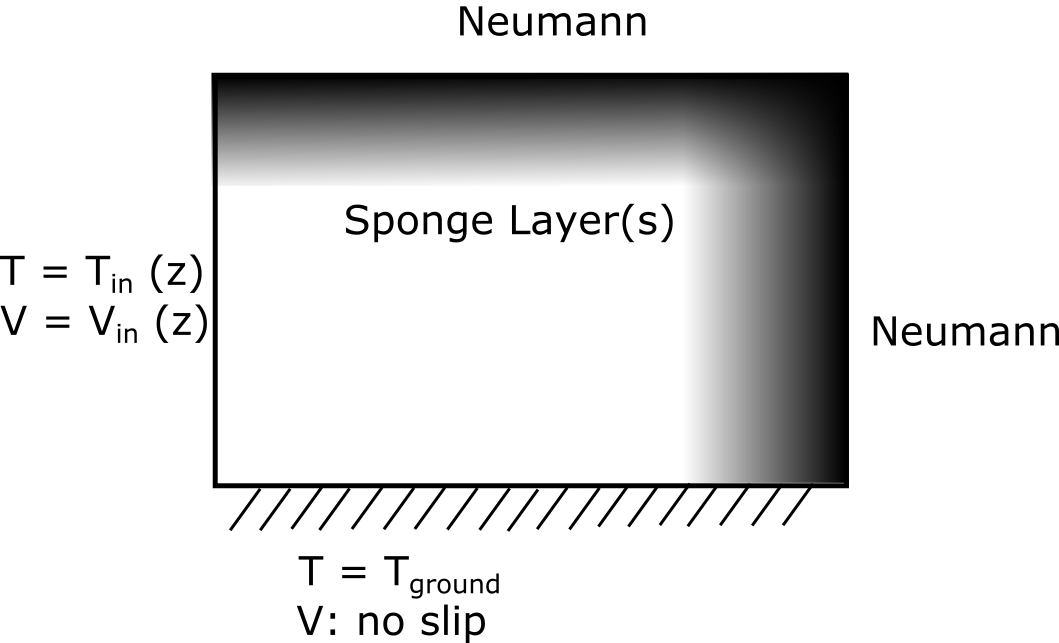
\includegraphics[width = 8 cm]{figs/wind_streamwise}
    \caption{Boundary conditions for the wind and thermal scenario, in
   the streamwise direction.} 
    \label{fig:windstream}
  \end{center}
\end{figure}

\begin{figure}[!htb]
  \begin{center}
    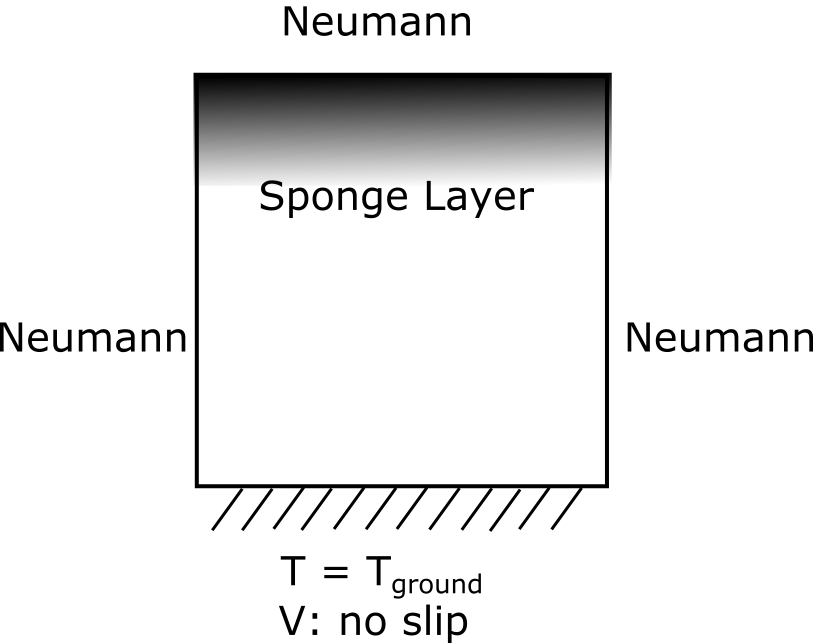
\includegraphics[width = 8 cm]{figs/wind_spanwise}
    \caption{Boundary conditions for the wind and thermal scenario, in
   the spanwise direction. } 
    \label{fig:windspan}
  \end{center}
\end{figure}

\subsection{Solver Options}

Solver options in Petsc\todo{finish me}
%% (11:40:27 AM) nick: ok so I don't understand what the option -sub_pc_factor_levels is
%% (11:40:42 AM) nick: what levels in the preconditioner am I setting?
%% (11:40:55 AM) Paul Bauman: sub = the preconditioner for the processor local solver
%% (11:40:58 AM) nick: petsc docs arent helping me
%% (11:41:01 AM) Paul Bauman: instead of the whole
%% (11:41:24 AM) nick: so if I set -sub_pc_factor_levels 0 is it not preconditioning, or just globally preconditioning the matrix?
%% (11:41:31 AM) Paul Bauman: Post all the options, it'll be easier to explain
%% (11:41:39 AM) nick: sorry im being daft, but i dont get it
%% (11:41:40 AM) nick: sure
%% (11:41:53 AM) nick: most I'm comfy with
%% (11:41:54 AM) nick: ``-ksp_view -ksp_type gmres -pc_type bjacobi -sub_pc_type ilu -sub_pc_factor_levels 0''
%% (11:42:00 AM) Paul Bauman: OK
%% (11:42:17 AM) Paul Bauman: -pc_type is the preconditioner for the entire linear system
%% (11:42:25 AM) Paul Bauman: You're doing bjacobi = block Jacobi
%% (11:42:28 AM) nick: right
%% (11:42:36 AM) nick: and does anyone have a good reference I can learn this better? i feel as if I cant look this up, for some reason
%% (11:42:39 AM) Paul Bauman: That is just using the inverse of the diagonal block for that processor
%% (11:42:46 AM) Paul Bauman: Now
%% (11:42:55 AM) Paul Bauman: that is a linear solve
%% (11:43:17 AM) Paul Bauman: So you can use all the linear solver technology to solve or approximately that block
%% (11:43:24 AM) Paul Bauman: Hence, -sub_pc_type
%% (11:43:32 AM) hil left the room.
%% (11:43:46 AM) Paul Bauman: That's the preconditioner it's going to use to precondition the linear system for the solution of the diagonal block
%% (11:43:53 AM) Paul Bauman: You're telling it to use incomplete lu
%% (11:44:26 AM) Paul Bauman: Now the -sub_pc_factor_levels options applies to ilu
%% (11:44:28 AM) hil entered the room.
%% (11:44:44 AM) Paul Bauman: The incomplete part of imcomplete LU is about the level of fill you use
%% (11:45:05 AM) Paul Bauman: The more levels of fill you have, the more ``complete'' the incomplete LU will be
%% (11:45:08 AM) Paul Bauman: Does that make sense?
%% (11:45:23 AM) nick: no, that is where you lost me
%% (11:45:39 AM) nick: i dont think i know this level of fill
%% (11:46:17 AM) Paul Bauman: Check out Youssef Saad's book if more curious about the subject
%% (11:46:37 AM) nick: cool thanks
%% (11:46:38 AM) Paul Bauman: Suffice it to say, you heopfully shouldn't ever need to go past 3 or 4 levels of fill
%% (11:47:03 AM) Paul Bauman: Also, if you've got superlu installed with the PETSc, consider using -sub_pc_factor_mat_solver_package superlu
%% (11:47:15 AM) Paul Bauman: That's a *much* faster/better implementation than PETSc's


\subsection{Software Stack}

The numerical approximations described above were implemented using the
GRINS library\cite{GRINSpaper} in Libmesh\cite{libMeshPaper}. 
It was designed to support multiphysics FEM
applications, the reusability and extensibility of mathematical
modeling kernels, supporting interfaces to existing solver and
discretization libraries to enable modern solution strategies, while, at
the same time, retaining flexibility to effectively address a wide range
of science or engineering problems. 

GRINS provides a platform that enables powerful numerical algorithms
such as adjoint-based AMR, adaptive modeling, sensitivity analysis,
and, eventually, enabling uncertainty quantification. While few of these
capabilities are in use for the present work, they could be useful in
future investigations. 

GRINS stands for, ``General Reacting Incompressible Navier-Stokes'',
which roughly encapsulates the physical regimes it was originally
designed to simulate. GRINS is open-source, and available on
\hyperref[www.github.com/grinsfem/grins]{github}. It is released 
under LGPL2.1.  GRINS is heavily unit tested, with over 60 tests
available to ensure the reliability of results regardless of install platform.

%The remainder of this subsection is devoted to
%discussing the underlying libraries used and the description of the
%GRINS framework.  
% PETSC\cite{petsc} trilinos\cite{trilinos}

% GRINS also uses the fparser\cite{fparser}
% library to support both parsing and compilation of mathematical
% functions into high 
% performance kernels. This capability allows for easy specification of
% boundary conditions, initial conditions, or constitutive equations from an input file. 

% Currently, libMesh has been scaled tens of thousands of cores and has
% been run on over 100,000 cores on the BG/Q machine Mira at Argonne National
% Lab\cite{libmesh-scaling}

%In principle, alternative software libraries/frameworks such as
%FEniCS\cite{fenics}, OpenFOAM\cite{openfoam}, etc. would likely be
%capable of simulating this regime. 


\subsection{Tool Chain and Simulation Custodianship}

Runs are queued on Texas Advanced Computing Center (TACC)
supercomputer's Lonestar Four and Stampede. Run durations are typically  
twelve hours to perform several hundred timesteps. 
These runs are generally submitted to the production queue and are  
264-528 processing cores, 
or 22-44 nodes on Lonestar (with 12 cores per node), and a similar number
for Stampede. The runs typically have several million degrees of freedom (DoF), 
and the local number of DoF per core is maintained at $O(10^4)$. This was
selected due to memory considerations, after a strong scaling
analysis of the performance of the code on these resources, and
after consulting with the software developers.  

After a run terminates, several scripts are automatically invoked. 
These scripts archive the run (outside of the volatile /scratch 
production directories) and simultaneously, label the concluded run with
unique metadata that defines the system environment, the jobs input
files and run definitions, as well as information detailing the
hypothesis or physics the job was intended to investigate. Finally, once
a week a script performs \textbf{rsync} on the entire archived database to
ensure more than single redundancy for the runs. 

In other words, the workflow is sufficiently advanced as to permit
rapidly queuing a series of runs (in parallel) to
investigate a variety of conditions or scenario parameters. This
capability is necessary for the optimization campaign detailed in
\ref{sec:proposed_work}, where running many concurrent investigations
will be required to adequately sample the configuration space. 


 
\section{Validation}
\label{sec:validation}


\begin{figure}[h]
 \begin{center}
  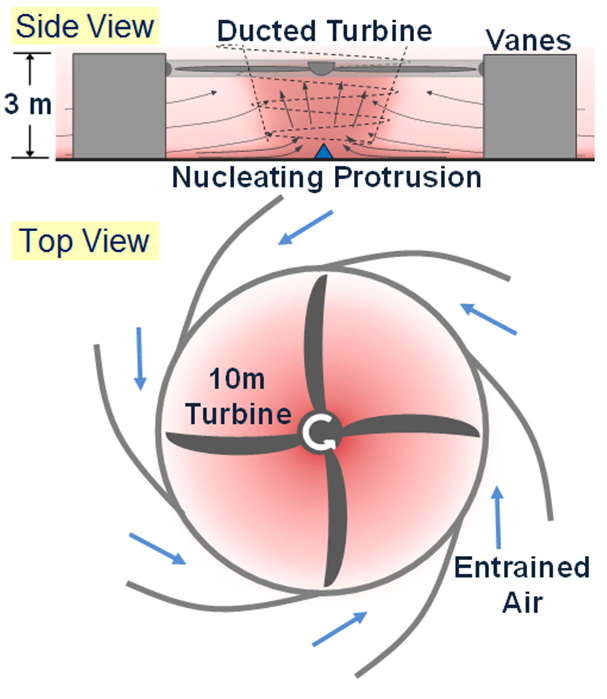
\includegraphics[width=.5\linewidth]{figs/power_generation.png}
   \caption{The Sov facility, showing the vanes, rotor and anchoring
   protrusion, as well as the buoyancy-driven vortex used to drive the
   turbine.}
   \label{facility}
  \end{center}
\end{figure}

The simulations are designed to both mimic the notional SoV experimental
facility as well as identify optimal configurations for future
designs. The general system configuration is depicted in Figure
\ref{facility}. 

Notice several important components of this device. First, ``vanes''
along the sides of the apparatus, designed to entrain outside air and
impart angular momentum. It is not known what configuration and design
of these vanes will lead to optimal dust-devil generation. Thus, these
vanes may have various configurations, varying in the number used, the
length, height, angle of attack. The vanes may also be straight, or
curved.  Next, the ducted turbine above the flow is also a critical design
component. This turbine is designed to extract energy from the flow,
without distrupting/destroying the vortex. Finally, it is desirable to
economically optimize the entire configuration scale by considering both
the power generation, cost of materials, difficulty and expense of
maintainance, etc. 

The model inputs consistitute a very large component (arguably, the
largest source) of the uncertainty in this problem, for both the
laboratory and outdoor test cases. For brevity, we consider here only
the laboratory cases. 

  \begin{figure}[!htb]
    \begin{center}
     \includegraphics[width = 12 cm]{figs/lab_setup.jpg}
     \caption{The laboratory set-up.}
     \label{lab}
    \end{center}
  \end{figure}

The experimental laboratory has numerous objects
in the immediate vicinity (see figure \ref{lab}) that may
obstruct/manipulate the flow. These objects may be moved or removed
during PIV data gathering. The laboratory simulation uses adiabatic side
walls as a boundary condition. It is unclear how much of an impact this
may have on the simulation. It is also unclear if this is a realistic
boundary condition. 

While no sensitivity analysis has been performed, it is likely that the
largest uncertainty in the laboratory simulation is a result of the
ventilation. This statement can be made because it was observed that the
heated plate on the bottom of the laboratory generated enough heat that
the room temperature began to rise significantly (30+ degrees
Celsius). This also greatly impacted the SoV performance, as the ground
to air thermal gradient drives the vortex. The laboratory uses cooling
in order to maintain temperature. They utilize two inlet HVAC ducts into
the room. While efforts have been made to characterize the level of
ventillation being used, these numbers come with non-trivial
uncertainties attached. As an example, a personal communication with one
of our experimental colleagues, 

``One vent runs continuously at 15 C with a flow rate of about 1
$m^3$/s (4-6 m/s with an approximate area of 0.2 $m^2$).''
Already, the inflow rate has a 50\% uncertainty in velocity
attached. Furthermore, while the area of the vents are given, the the
precise height and width are not. Thus, while our simulation uses square
vents, this may be inaccurate. 
It was also stated that, ``The other vent kicks on only if the
room gets about 28 degrees C.'' This statement has uncertainty attached to the
temperature at which the venting begins. Finally, ``The exit air is just
what ever leaves through/around the doors as we've blocked off all of
the out ducts.'' This also presents a challenge, as it is unclear (for
validation purposes) where one should expect the outflow to
go. \footnote{\normalsize Author note: This story related here not as a comment on
our collaborators. Rather, this is presented as an example of the challenges
and uncertainties that presently exist in this numerical investigation.}

We impose Dirichlet boundary conditions to establish a constant inflow
condition of cool air at the rates proscribed by our
collaborators. Unfortunately, we have found that the using inflow rates
consistent with the lower bound of those estimates result in an
unrealistic heating of the room, while inflow conditions at the high end
result in velocity profiles that exceed the laboratory measurements. In
other words, our simulations appear to be sensitive to the choice of
inflow rate, and it is likely that the laboratory is run where one of
the vents is operating intermittently. 

The initial conditions in both the laboratory and the outdoor
tests are highly uncertain. The dimensions of the laboratory are
(it is presumed) measured with a high degree of confidence, however, the
initial temperature 
in the room is not closely measured, and may vary as a function of
time or across tests. We note however, that the solutions from the simulations are
generally stationary in time, and consistent results are gathered from several
simulations with different initial conditions. Therefore, it does not
appear that the initial conditions in the room in terms of the ambient
velocity or temperature field are a large source of uncertainty in the
laboratory.

\subsection{Model Calibration}

%
% viscosity calibrated
% 


\subsection{Challenges}

Several phases of research must be conducted in order to develop robust
and reliable predictive simulation capability. First, the simulations
must be validated against existing experimental data generated from the
laboratory apparatus. These data were taken using particle image
velocimetery (PIV), often not without non-trivial error in measurement and
sampling. Finally, as mentioned previously, the measurements for the
cooling, geometry of the room, etc. are rough, and almost certainly
possess non-trivial uncertainties/errors. As a result, this is already a
difficult validation scenario. 

The validation challenge is compounded by the fact that very little is
known about the uncertainties in the observation data. PIV is a
non-intrusive technique, but it does rely upon large sample sizes in
order to generate reliable statistics. While several hundred PIV
snapshots are available, no quantified uncertainties for the averaged fields
presently exist.  

In addition, only velocity measurements are available. Several
potentially important quantities of interest, such as the pressure field
or the temperature, have not been measured, and cannot then be used for
the purposes of validation. This presents a risk that our 
simulations might generate acceptable velocity fields, but that a
significant source of error may exist in unobserved QoIs, and would not
be detected in our present validation regime. 

Furthermore, the model form in use is known to be imperfect. 
Model inadequacy may play a significant role in both the validation
scenarios described below, as well as (more chillingly) in the
additional regimes that the models will be used in a predictive
capacity. 

\subsection{Model Validation}
Our initial focus has therefore moved to a validation study to ensure that the
output of the numerical simulation agrees with the experimental
measurements. The flows are qualitatively similar, with a vortex forming
in the center of in both cases, but the degree to which each matches
each other is unclear and must be characterized. 

\begin{figure}[!htb]
        \centering
        \begin{subfigure}[bh]{0.5\textwidth}
                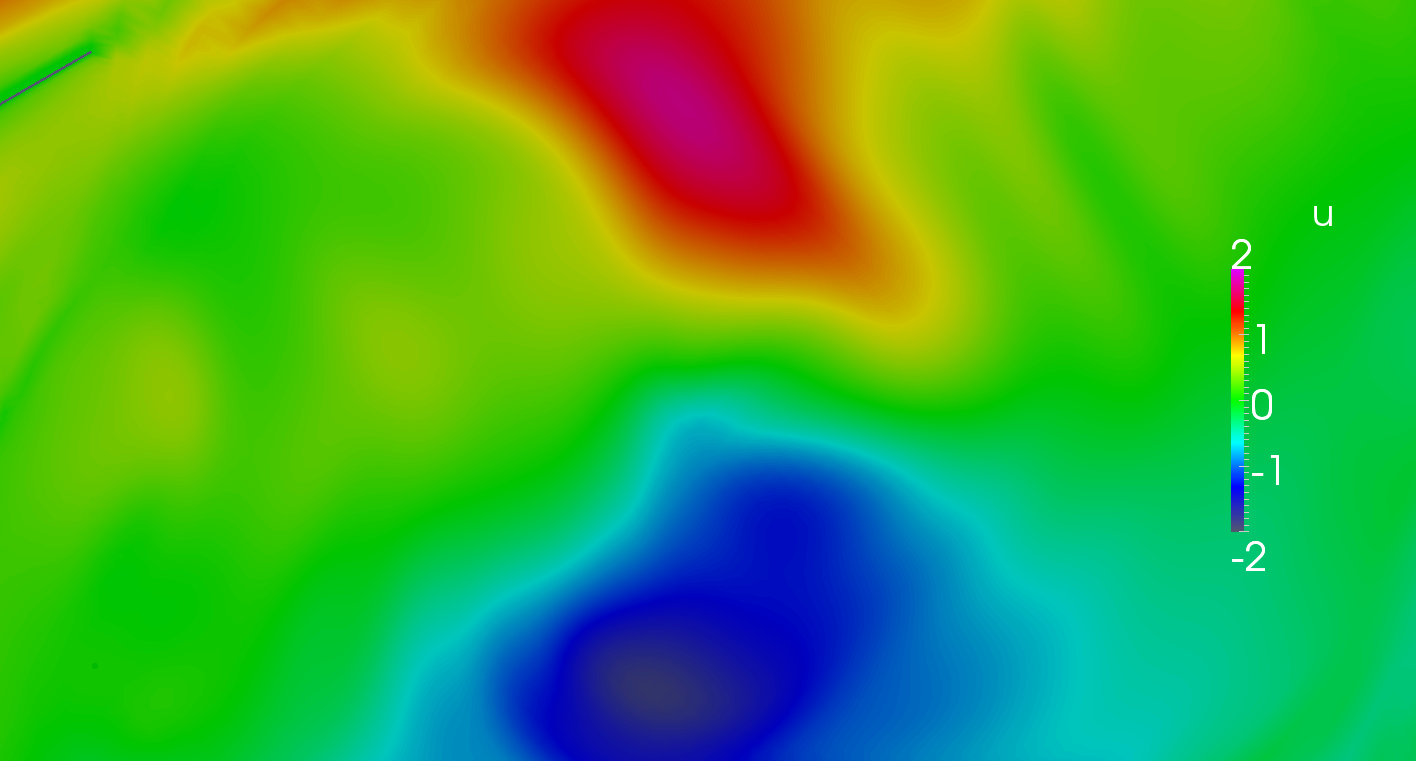
\includegraphics[width=.8\linewidth]{figs/u_sim.png}
        \end{subfigure}%
        \begin{subfigure}[bh]{0.5\textwidth}
                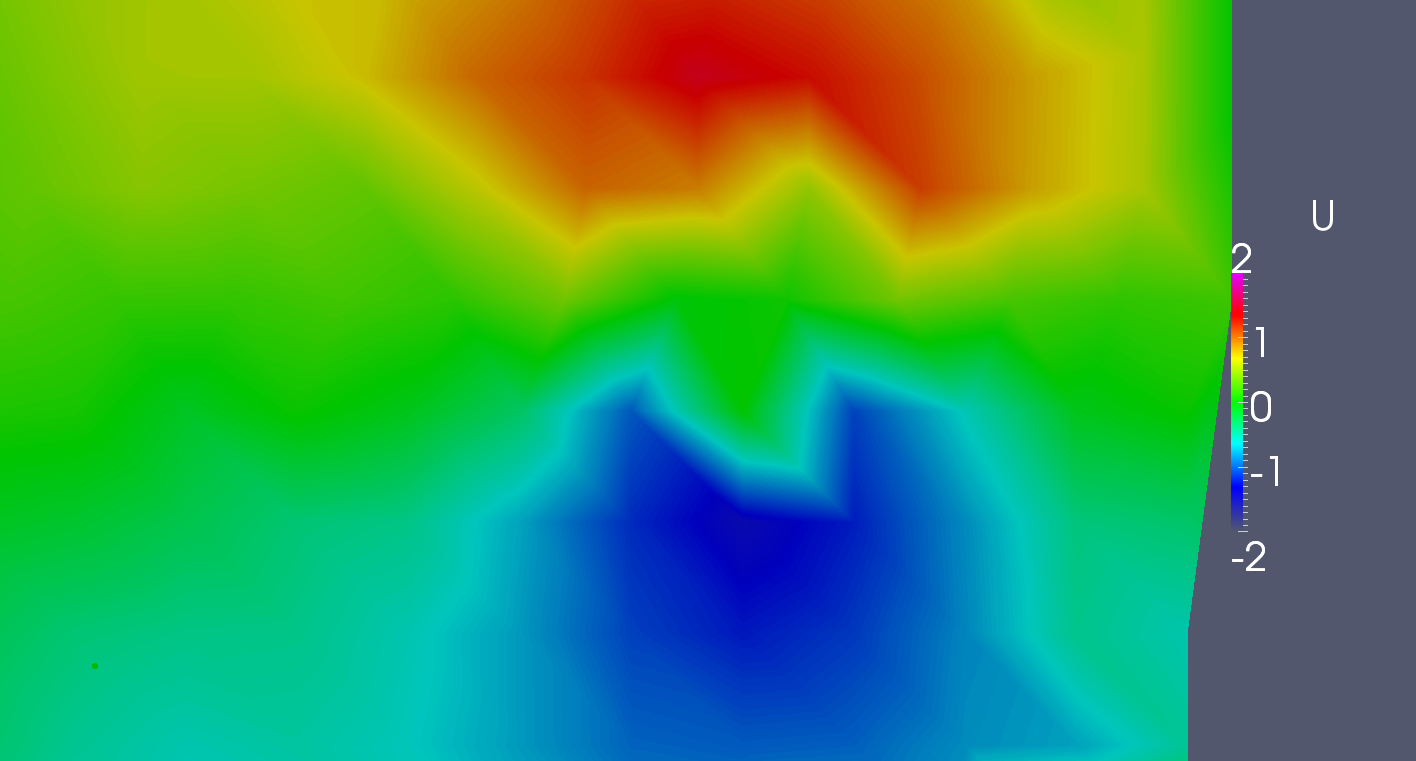
\includegraphics[width=.8\linewidth]{figs/u_exp.png}
        \end{subfigure}
 \caption{The instantaneous x velocity component (u)
 from a horizontal plane situated slightly above the vanes,
 measured in the simulation (left) and the laboratory apparatus
 (right). This is for a 30 degree vane configuration.} 
 \label{fig:instant}
\end{figure}


In particular, we have implemented a simulation designed
to closely mimic the 30 degree vane experimental setup. The outputs of
the simulation (velocity field, temperatures, etc. ) are then compared
to available experimental data, which at this time is principally the
velocity field taken by PIV measurements at a variety of time frames
near the center of the SoV. This ``high-cost'' simulation resolves
the SoV large-scale structure, as well as the turning vanes
nearby. Comparisons must be made between the:
\begin{itemize}
 \item Azimuthal Velocity as a function of radius from center of the Sov
 \item Azimuthal Velocity as a function of the height at different
       points in the SoV
 \item Vertical Velocity as a function of radius from center of the Sov
 \item Vertical Velocity as a function of the height at different
       points in the SoV
\end{itemize}
As noted above, this is an extremely limited set of comparisons. 

%
% hybrid (embedded model)
%
Further validation cases are required. We are now in a position to perform
a validation of the embedded vane model. As described previously, this
uses the same turbulence models, but now without resolving the turning
vanes. Instead of resolving the vanes, for a region in the flow, the
velocity field is forced in a manner similar to as if the fluid was
moving through the turning vanes. While direct comparisons between this
model and the experimental data can be (and will be) made, a comparison between this
``low-cost'' (in terms of computation and mesh requirements) simulation
and is useful for several reasons. It permits directly comparing the effect of
the simple, low cost, turning vane model against the higher resolution
modeling (essentially this permits a validation of an embedded
model). Furthermore, it allows us to observe a much richer set of
possible changes in the state space than in the experiment, which is
constrained to only velocity measurements. 

%
% 7) An assessment of what further concerns might remain after (5) and
%   (6) regarding the applicability of the model for the purpose of the
%   calculations.
%
\section{Further Concerns}

% the fucking turbine too...
Our goal is to eventually extract energy from the SoV, which at this
time is envisioned coming from a turbine placed over the vanes. It will
be very difficult to get accurate PIV measurements from the apparatus in
the laboratory, and once again the simulations will be essential in
driving the experimental optimization and design of the SoV. Thus, 
this adds another significant validation case, with new, significant,
challenges in modeling the turbines. This is in essence a new embedded
submodel that we will add after validation of the initial configuration
is completed. 

In order for these simulations to be generally useful, after they are 
validated against existing experimental data and high fidelity
simulations, they will be used to explore regimes and scales where no
experimental measurements presently exist. Characterizing the
uncertainty of predictions resulting from extrapolation is a critical
component in enabling reliable assessments of field performance of the
SoV, as it will guide the commercialization strategy of the product.

% scaling analysis
These new simulations at different conditions will be performed in order
to inform the optimal design and scale of the planned two and five meter
SoV prototypes, to be installed in Arizona. This study will inform the
design based on the scaling of the velocity field and anticipated energy
generation. Furthermore, insights may be gathered on the dyamics of
these flows, which could lead to fundamental advances in the physics of
fluid dynamics, dust devils, and other coherent structures with vortex 
dynamics\cite{Mullen1977181,smithleslie,kanak}. 

% this might be junk
Determining the optimal design of these systems will involve parameter
sweeps over a large space of possible configurations. These simulatons
are expensive, and so while accuracy is important, where possible,
models will be developed in order to simplify the mesh (memory) and
computational requirements. For instance, the previous ``low-cost'' vane
 method, which replaces the turning
vanes with a model, improved runtime by a factor of twenty-four, due to
the greatly decreased mesh resolution requirements near the vane
trailing edges. These models, if they prove to be robust after
validation testing, will be
invaluable tools in effective computer aided design and simulation of
this new technology.  


 
\section{Preliminary Results}
\label{sec:results}

%
% RESULTS TODO
%
% need to motivate optimization workflow and plans
% current ideas not bad, need more
%
%

The computer simulations in this proposal study are intended to discover
the optimal solar vortex system configuration for a range of scenarios
and system sizes. 
This section contains discussions of the preliminary simulation results 
to motivate that the existing simulation capability is sufficiently well
developed and understood to permit an efficient exploration of the SoV
configuration space. 
This section begins with a discussion of the structure of solutions from
a representative case with no ambient winds, the ``thermal only''
situation. Next, a case with strong ambient horizontal winds (``Wind'')
is discussed. Finally, the results from a series of runs are shown to
demonstrate heuristic by which incremental optimization of the system
configuration will be conducted. 

%The results of these optimized configurations will be used as input
%for the design of a prototype to be tested in Mesa, Arizona this
%summer. 

% \todo{add photo}
  % \begin{figure}[!htb]
  %  \begin{center}
  %   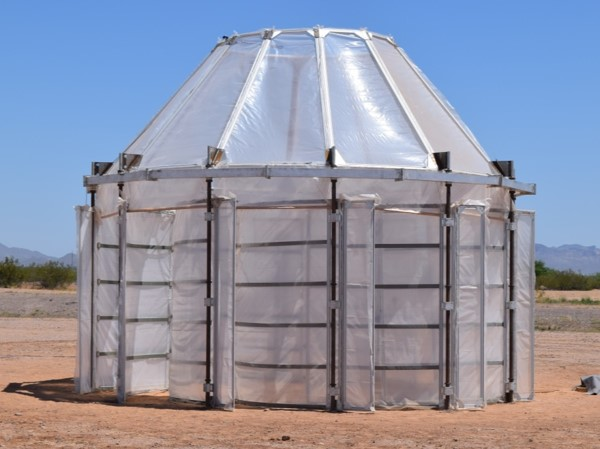
\includegraphics[width = 12 cm]{figs/sov_field}
  %   \caption{A photo of the field configuration, during the June 2015
  %   Field Test.}
  %   \label{fig:field_real}
  %  \end{center}
  % \end{figure}

\subsection{Thermal Only}

While ambient winds in the field impact system performance, it is
also illuminating to consider an idealized scenario with natural convection
driven only by thermal instabilities. Simulations of this baseline,
thermal-only flow are intended to ensure the SoV apparatus to form a
strong thermal plume even in the absence of wind. 
%After a system is
%engineered to form a strong thermal plume, we can investigate to ensure
%that the existing thermal vortex will be strengthened by the addition of
%winds. %\todo{do I need image of vanes? and explain how calculated}

\begin{figure}[htb]

 \begin{subfigure}{.55\textwidth}
  \centering
  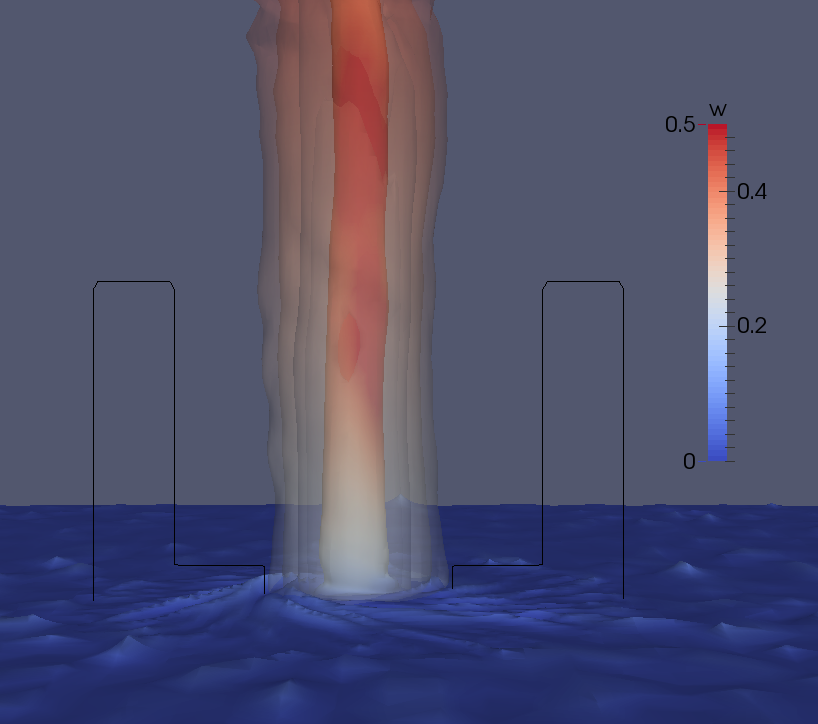
\includegraphics[width =0.7\textwidth]{figs/3d}
  \caption{Isocountours of the inner thermal core
  visible through semi-transparent contour around azimuthal velocity,
  colored by vertical velocity. An outline of the region of virtual
  vanes has been drawn.}
  \label{fig:thermal}  
 \end{subfigure}%
 \begin{subfigure}{.4\textwidth}
  \centering
  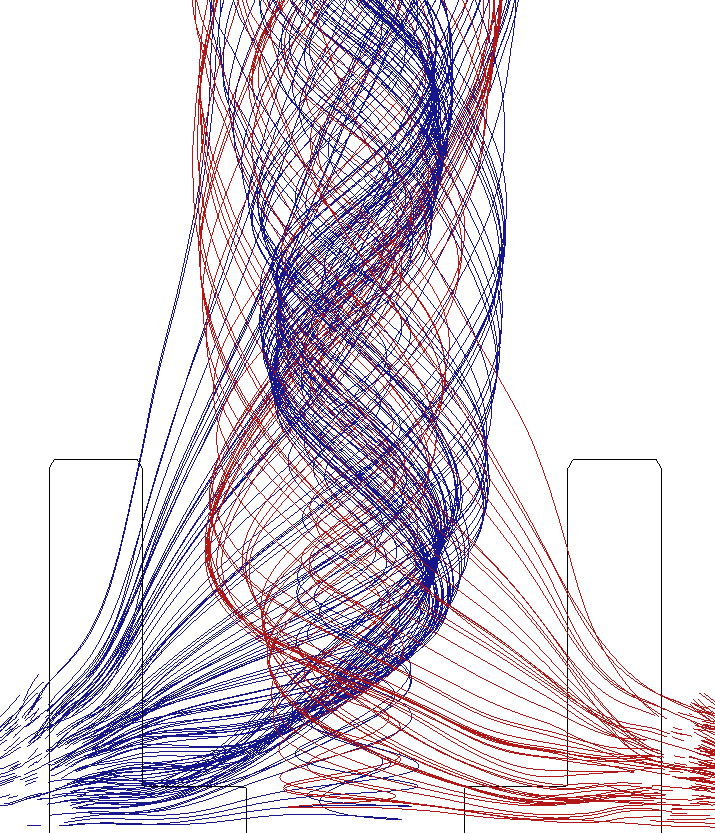
\includegraphics[width =0.8\textwidth]{figs/entrainment}%
  \caption{Fluid entrainment around the apparatus. An outline of the
  virtual vanes are drawn to show the region of forcing.} 
  \label{fig:entrain}  
 \end{subfigure}%
\end{figure}

In this subsection a representative case of an optimized thermal-only SoV
configuration is presented.\todo{what are the conditions of this case} 
The results shown are the averages of fifty snapshots of the solution 
taken over the course of ten minutes. In general,
the averaging times are selected to be approximately 20 to 30 wash-out 
times, where a
wash-out is defined as the time required for a particle at the base of
the apparatus to flow out through the top boundary. The energy flux
through the top of the vanes for this case is about 53 watts. The solution
demonstrates several features characteristic of naturally occuring dust
devils. Figure \ref{fig:thermal} shows that there is a tight,
coherent thermal plume roughly the same size as the inner diameter of the
lower vanes. As anticipated, this hot flow is acting like a chimney,
generating a large vertical velocity which in turn entrains air from the outside.
An image of the entrainment is shown in figure
\ref{fig:entrain}\todo{fix text of this image}. The image was created by
tracking particles as they convect through the device. 
One can observe a tight inner vortex with significant azimuthal velocity  
as well as a broader region of entraining fluid through the 
upper tier of vanes. 

\begin{figure}[htb]

 \begin{subfigure}{.5\textwidth}
  \centering
  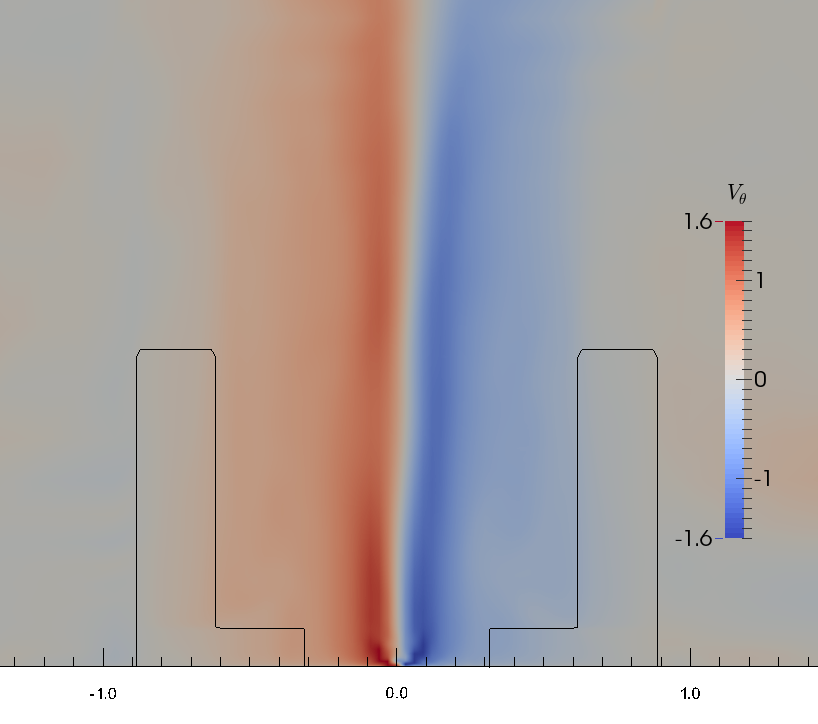
\includegraphics[width=.75\linewidth]{figs/vt}
  \caption{Azimuthal Velocity}
  \label{fig:vt-to}
 \end{subfigure}%
 \begin{subfigure}{.5\textwidth}
  \centering
  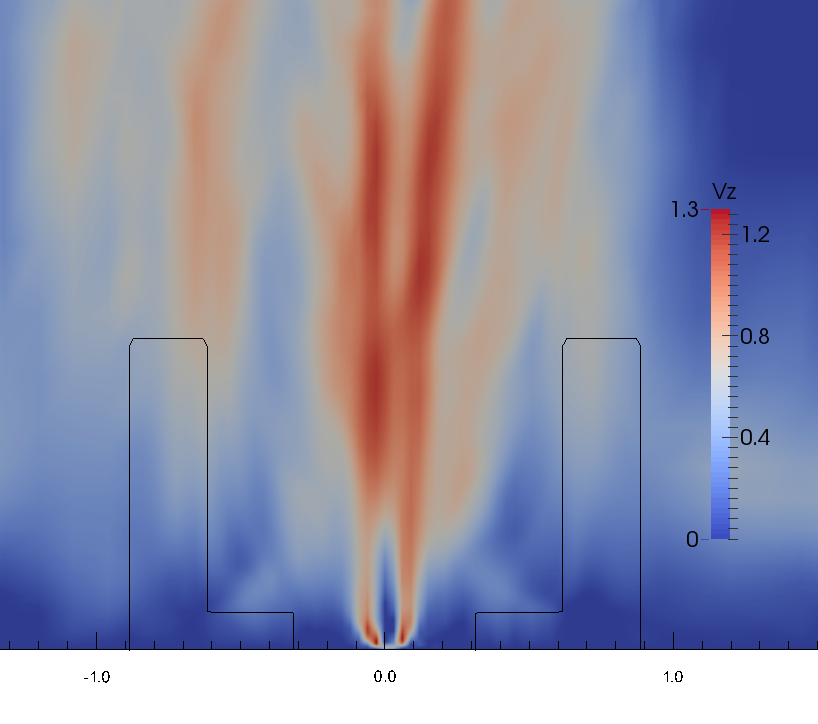
\includegraphics[width=.8\linewidth]{figs/vz}
  \caption{Vertical Velocity}
  \label{fig:vz-to}
 \end{subfigure}%


 \begin{subfigure}{.5\textwidth}
  \centering
  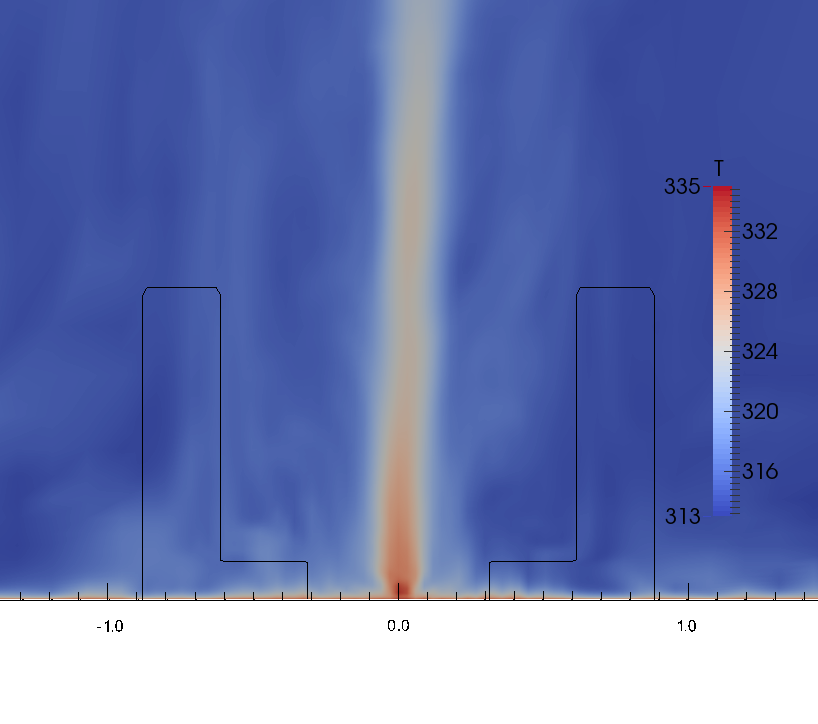
\includegraphics[width=.85\linewidth]{figs/t}
  \caption{Temperature}
  \label{fig:t-to}
 \end{subfigure}%
 \begin{subfigure}{.5\textwidth}
  \centering
  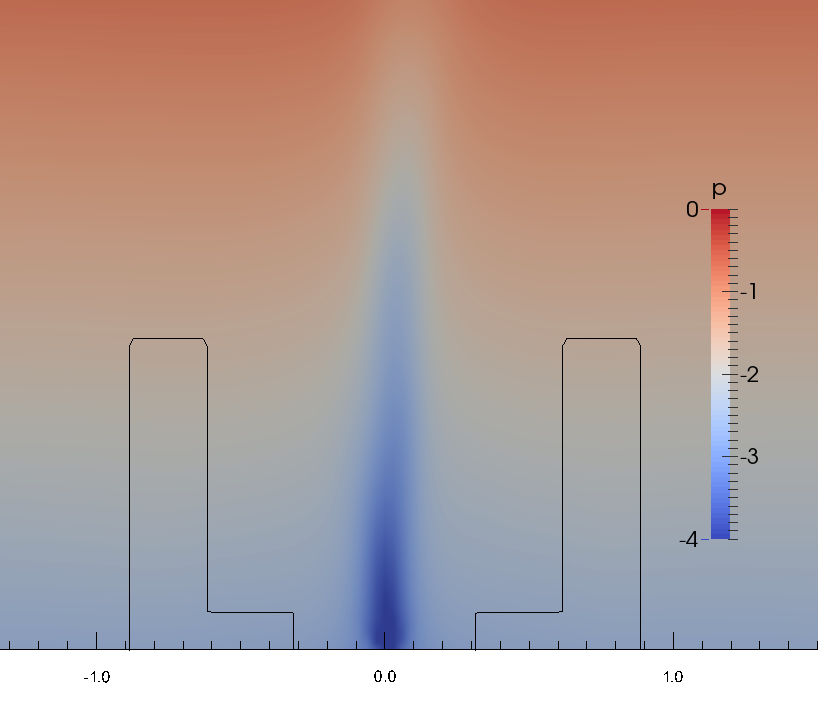
\includegraphics[width=.75\linewidth]{figs/p}
  \caption{Pressure}
  \label{fig:p-to}
 \end{subfigure}%

 \caption{Vertical slices through the center of the device for the thermal-only cases. Black lines 
   indicate the location of the vanes.}
 \label{fig:to-vert}
\end{figure}

%
%
%
Figure \ref{fig:to-vert} depicts several vertical slices through the SoV
for various state variables. One can see that there is a tight core
vortex with azimuthal and vertical velocities of several meters per
second. The tight vortex region coincides with a high temperature, low
pressure core region. The rapidly rotating air near the center induces
a low pressure core, as observed in real dust devils.
On the vertical velocity plot, notice that a small
downward flow region has formed in the middle of the vortex. 

\begin{figure}[htb]

 \begin{subfigure}{.5\textwidth}
  \centering
  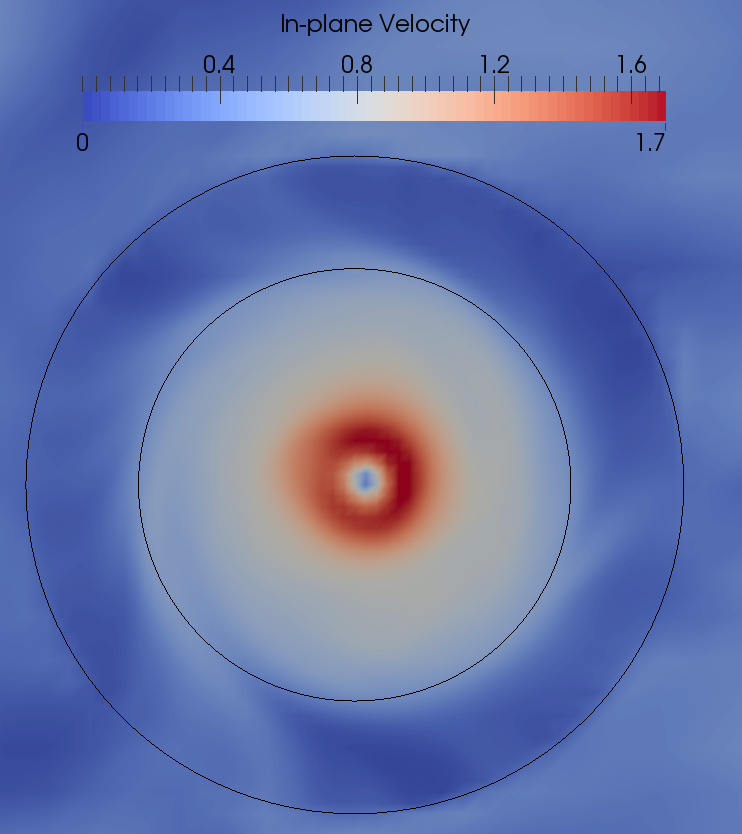
\includegraphics[width=.75\linewidth]{figs/vt_hor}
  \caption{Azimuthal Velocity}
  \label{fig:vt-to}
 \end{subfigure}%
 \begin{subfigure}{.5\textwidth}
  \centering
  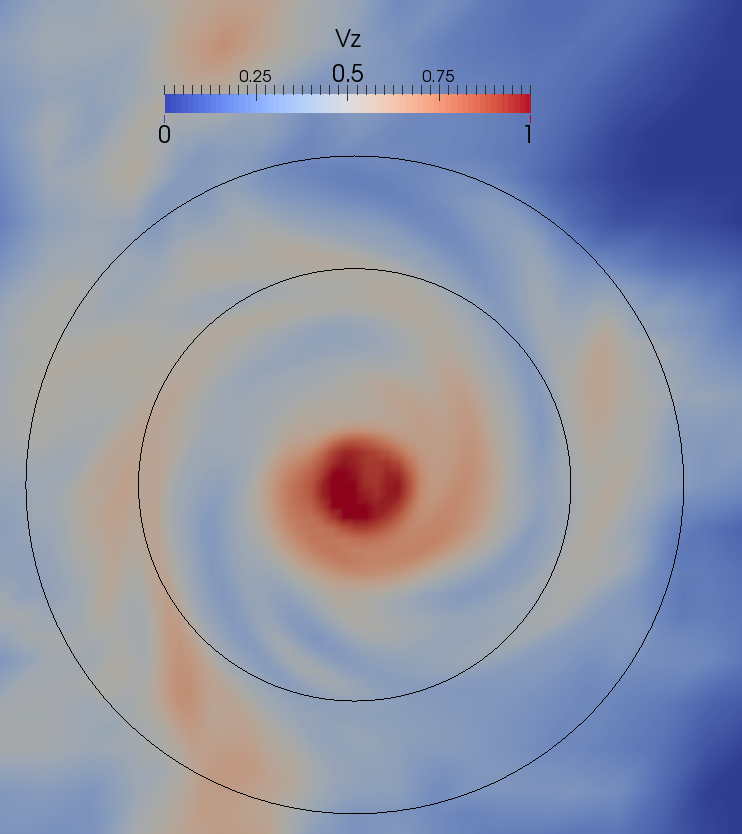
\includegraphics[width=.8\linewidth]{figs/vz_hor}
  \caption{Vertical Velocity}
  \label{fig:vz-to}
 \end{subfigure}%


 \begin{subfigure}{.5\textwidth}
  \centering
  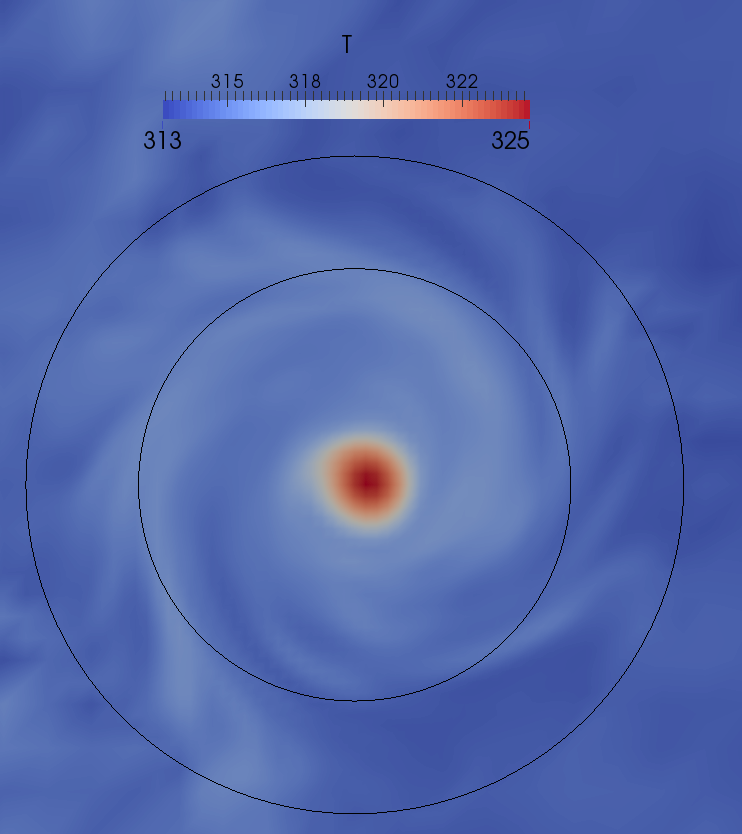
\includegraphics[width=.85\linewidth]{figs/t_hor}
  \caption{Temperature}
  \label{fig:t-to}
 \end{subfigure}%
 \begin{subfigure}{.5\textwidth}
  \centering
  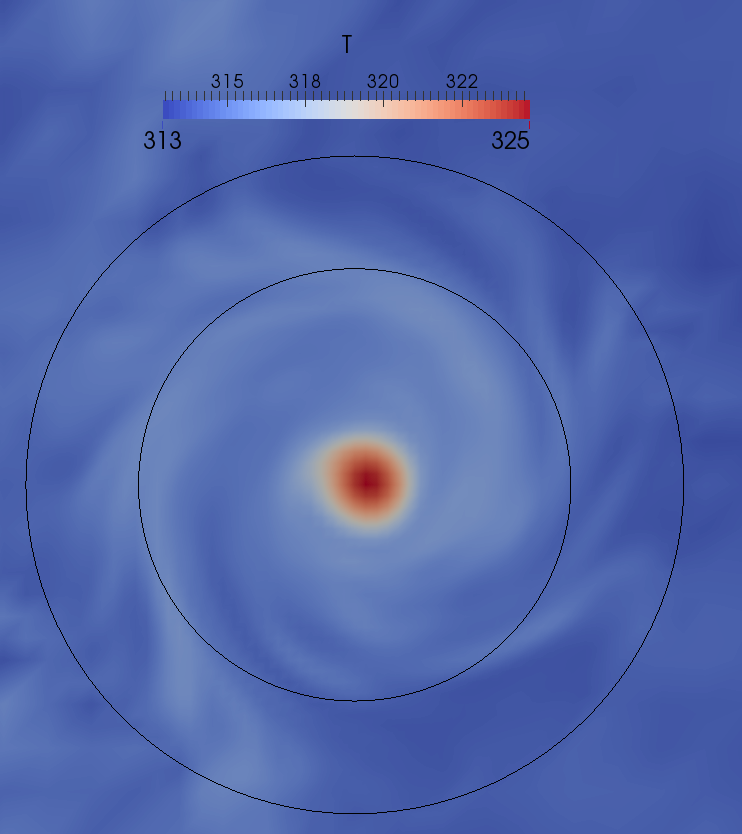
\includegraphics[width=.75\linewidth]{figs/t_hor}
  \caption{Pressure}
  \label{fig:p-to}
 \end{subfigure}%

 \caption{Horizontal slices for the thermal-only cases.}
 \label{fig:to-hor}
\end{figure}

Figure \ref{fig:to-hor}, depicts several horizontal slices
through the SoV for the same state variables. It can be seen that the
large velocities are highly localized to a region just inside the
vanes. Likewise, the entrainment of fluid is limited to a region
immediately surrounding the vanes. 
%
% conclusion of thermal only
%
Finally, the thermal plume is relatively
narrow compared to the diameter of the device. It is desirable to
broaden the thermal plume, as this would create a larger vertical
momentum flux and consequentally a larger kinetic energy flux. 
%% This will presumably
%% entrain more surrounding fluid, driving it through the vanes and
%% imparting kinetic energy to the flow. The kinetic energy grows as the
%% square of the radius, so any broadening of the vortex core can greatly
%% enhance the kinetic energy flux. 
The diameter of the thermal core is
therefore a critical flow characteristic in the thermal-only
conditions. However, a means of determing the thermal plume's thickness 
is not presently known. Regardless, these slices lend credibilty to the
notion that our turning vane configuration is generating something with
visible parallels to a naturally occurring dust devil.   

\subsection{Wind}

todo\todo{what case is this?}

%
% horizontal slices
%
\begin{figure}[htb]

 \begin{subfigure}{.5\textwidth}
  \centering
  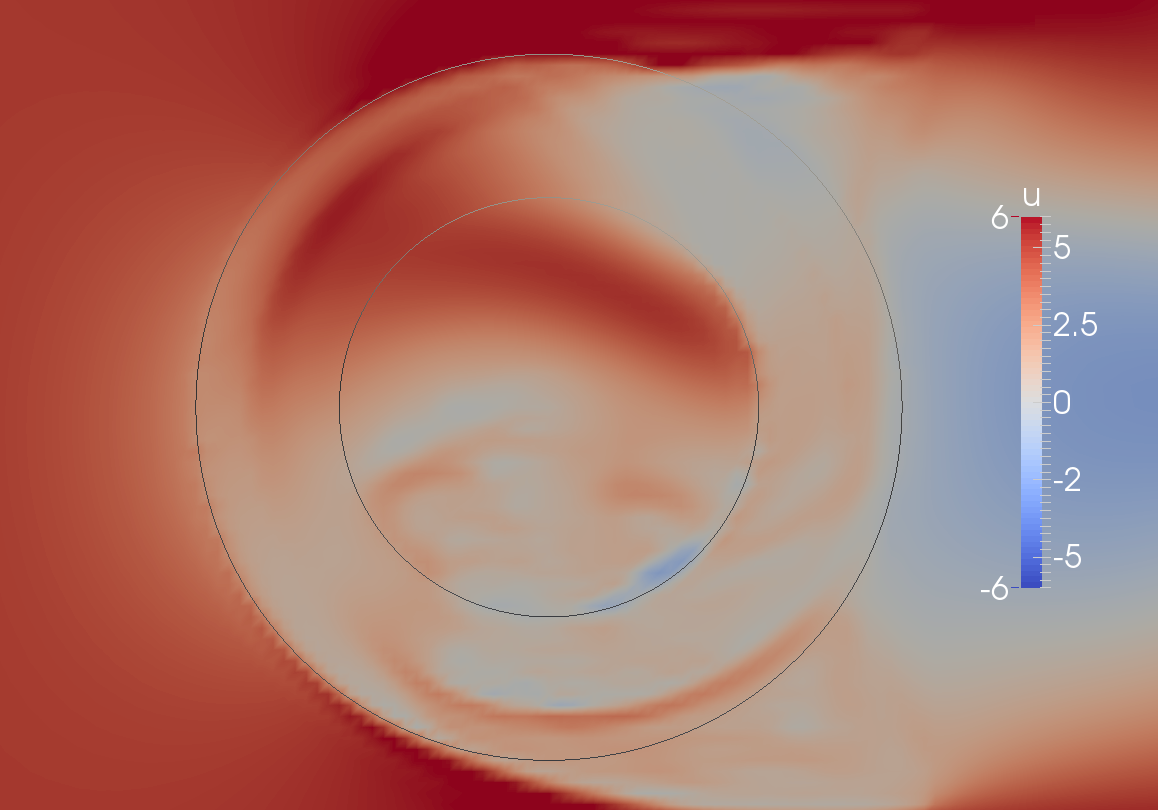
\includegraphics[width=.75\linewidth]{figs/wind_u}
  \caption{Streamwise}
  \label{fig:vt-wind}
 \end{subfigure}%
 \begin{subfigure}{.5\textwidth}
  \centering
  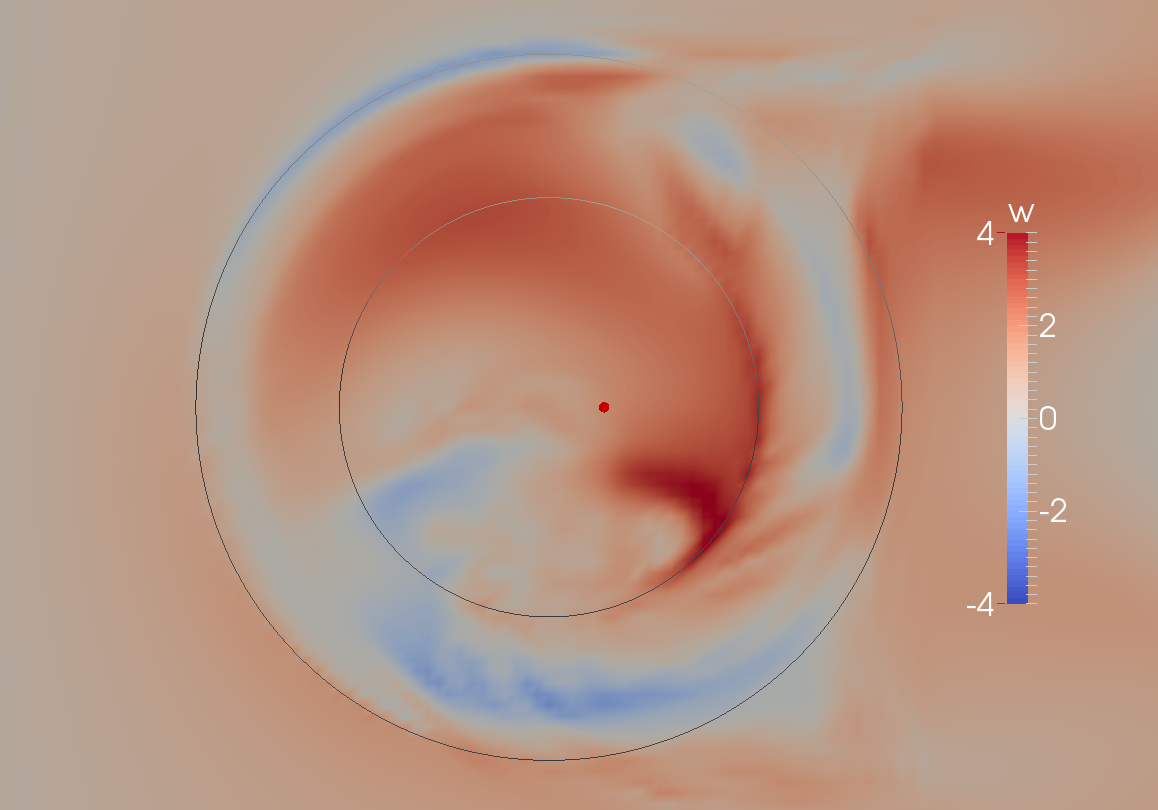
\includegraphics[width=.8\linewidth]{figs/wind_w}
  \caption{Vertical Velocity}
  \label{fig:vz-wind}
 \end{subfigure}%


 \begin{subfigure}{.5\textwidth}
  \centering
  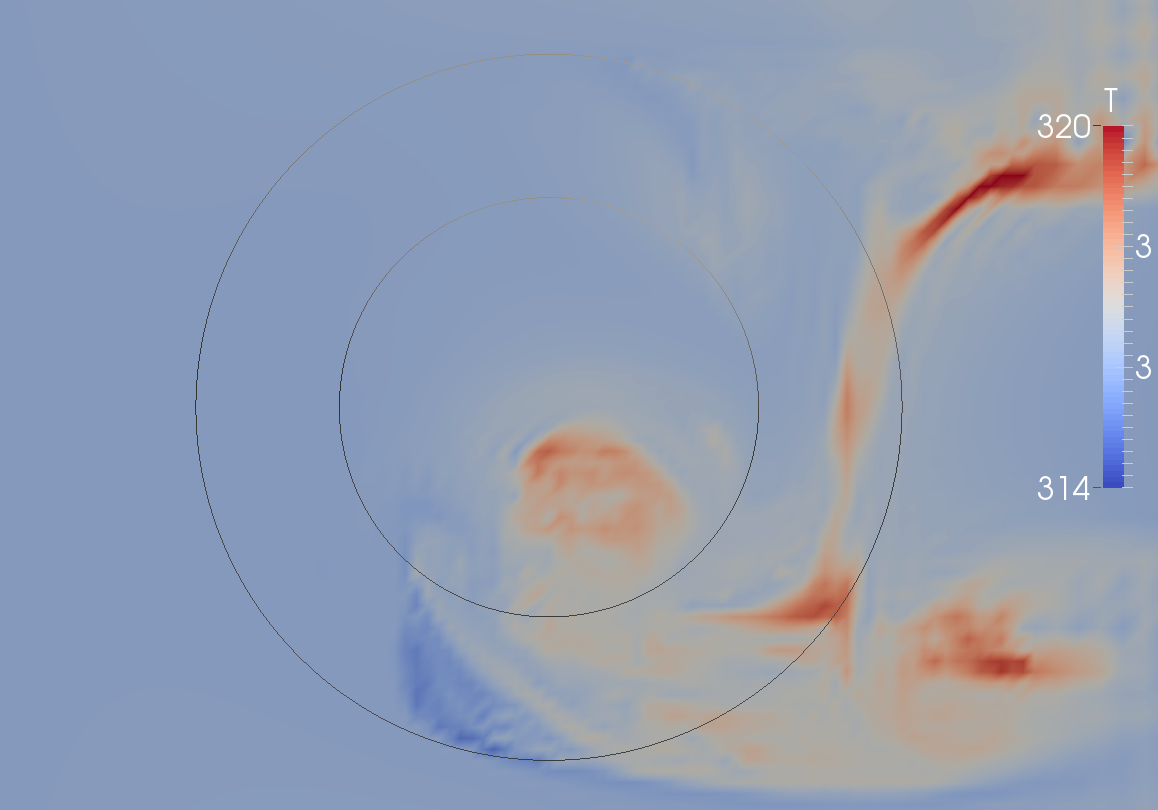
\includegraphics[width=.85\linewidth]{figs/wind_t}
  \caption{Temperature}
  \label{fig:t-wind}
 \end{subfigure}%
 \begin{subfigure}{.5\textwidth}
  \centering
  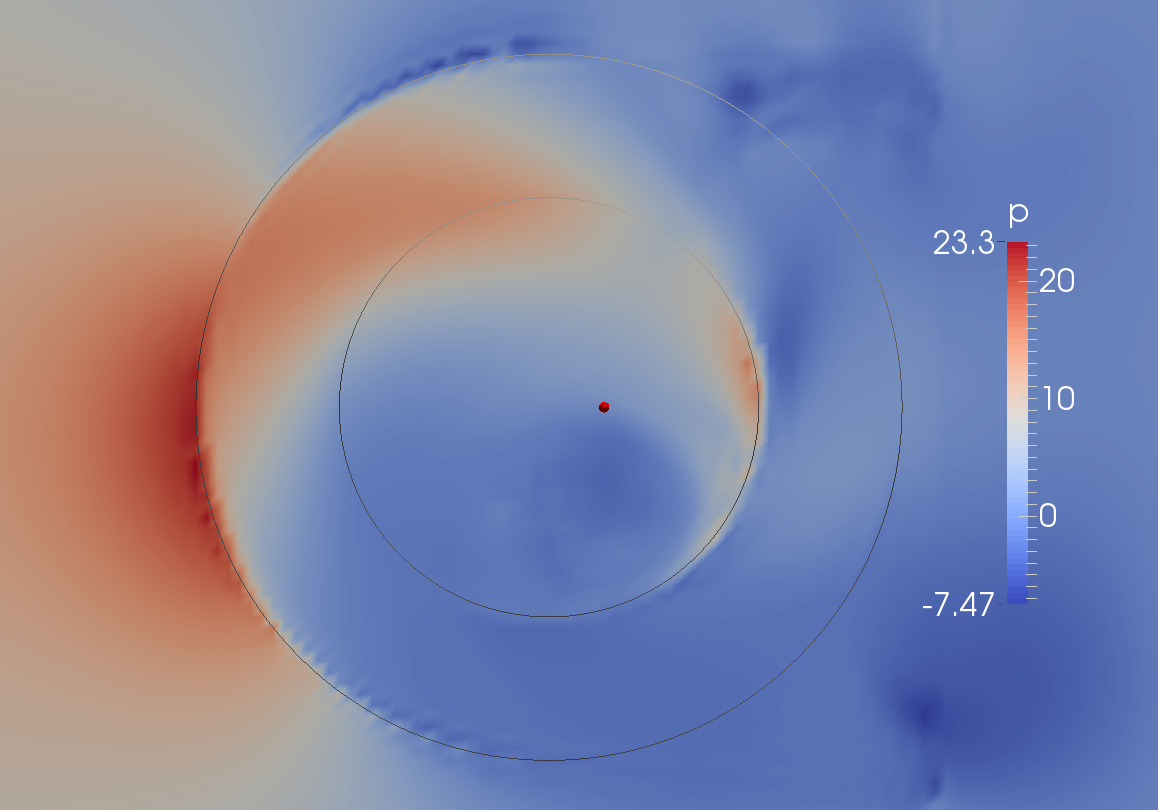
\includegraphics[width=.75\linewidth]{figs/wind_p}
  \caption{Pressure}
  \label{fig:p-wind}
 \end{subfigure}%

 \caption{Horizontal slices for the wind cases.}
 \label{fig:wind-hor}
\end{figure}


Horizontal slices of the azimuthal and vertical velocities, as well as the 
temperature and pressure fields are shown in figure \ref{fig:vz-wind-vert}. The freestream velocity
is traveling from left to right at $5 m/s$, which was set based on ambient velocity measurements made by 
the experimental team from the field. 
While the structure is undoubtedly different than the thermal-only cases shown previously, 
we can nevertheless see that a thermal plume is forming along with a 
rotating velocity structure. In general the wind cases are more disorganized, with less obviously 
visible coherent structure. Notice however that the magnitude of velocities are several times larger than 
in the thermal-only cases, and the kinetic energy flux through the vanes is also significantly higher. 

%
% vertical
%
\begin{figure}[htb]

 \begin{subfigure}{.5\textwidth}
  \centering
  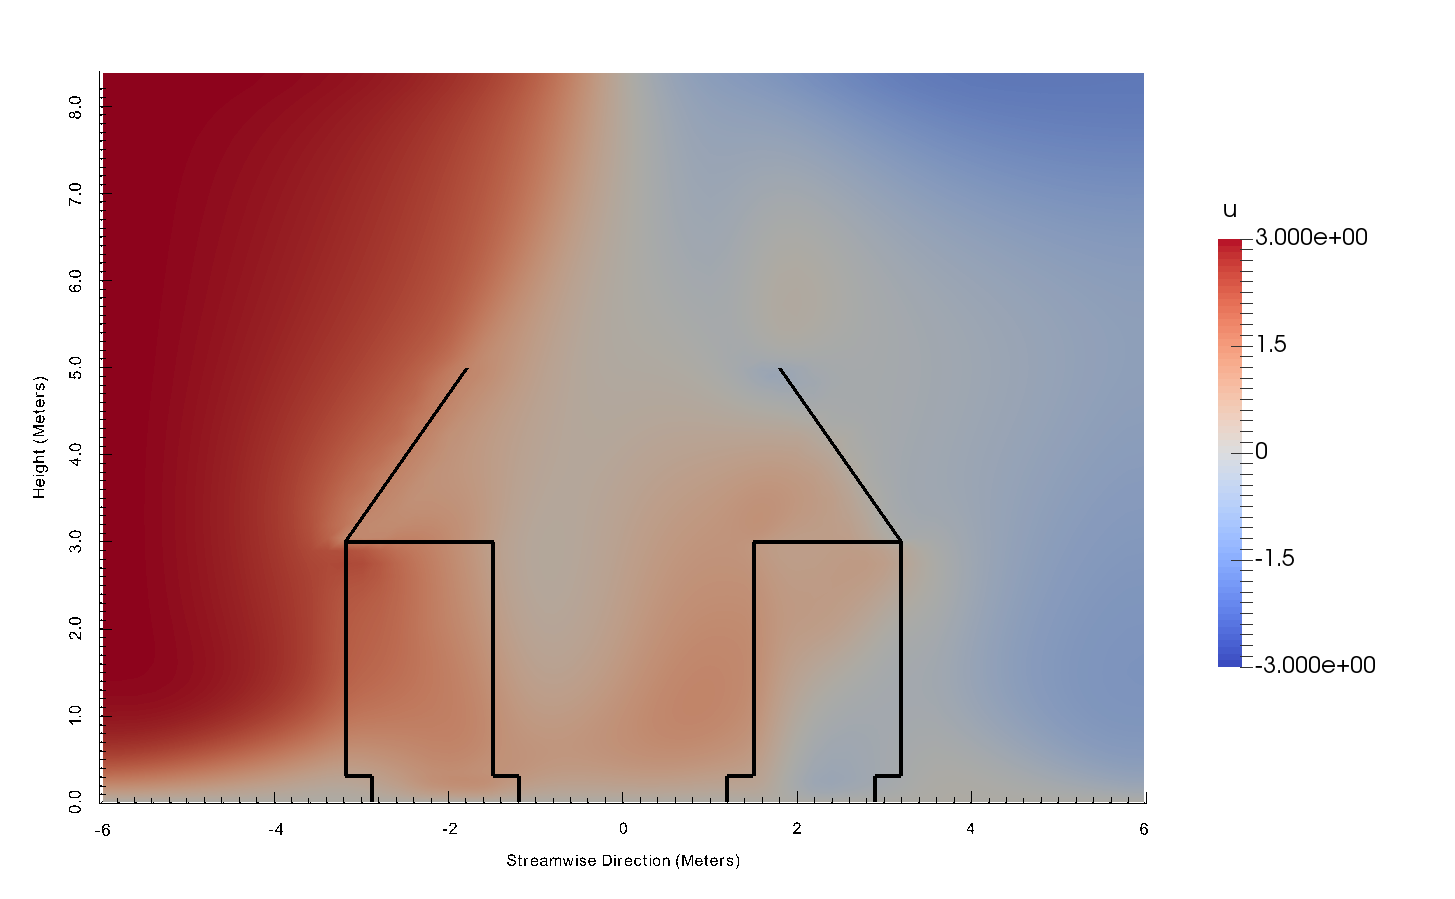
\includegraphics[width=.75\linewidth]{figs/wind_u_vertical}
  \caption{Streamwise}
  \label{fig:vt-wind-vert}
 \end{subfigure}%
 \begin{subfigure}{.5\textwidth}
  \centering
  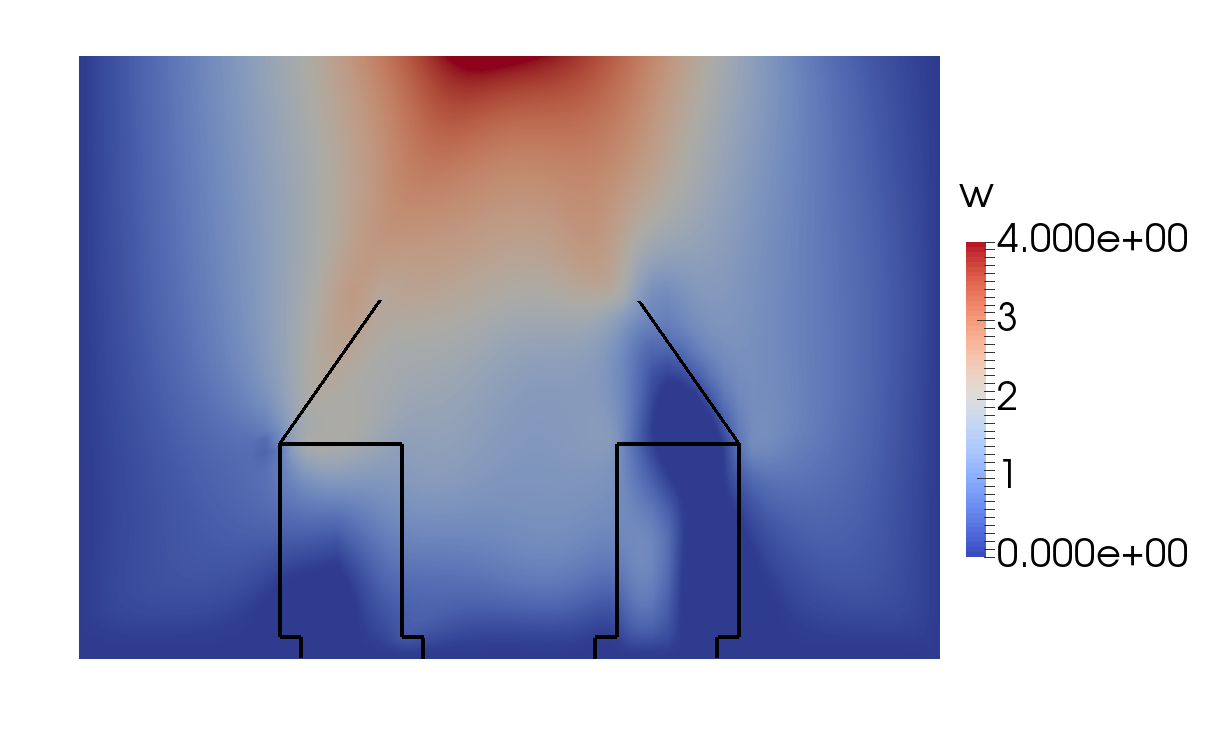
\includegraphics[width=.8\linewidth]{figs/wind_w_vertical}
  \caption{Vertical Velocity}
  \label{fig:vz-wind-vert}
 \end{subfigure}%


 \begin{subfigure}{.5\textwidth}
  \centering
  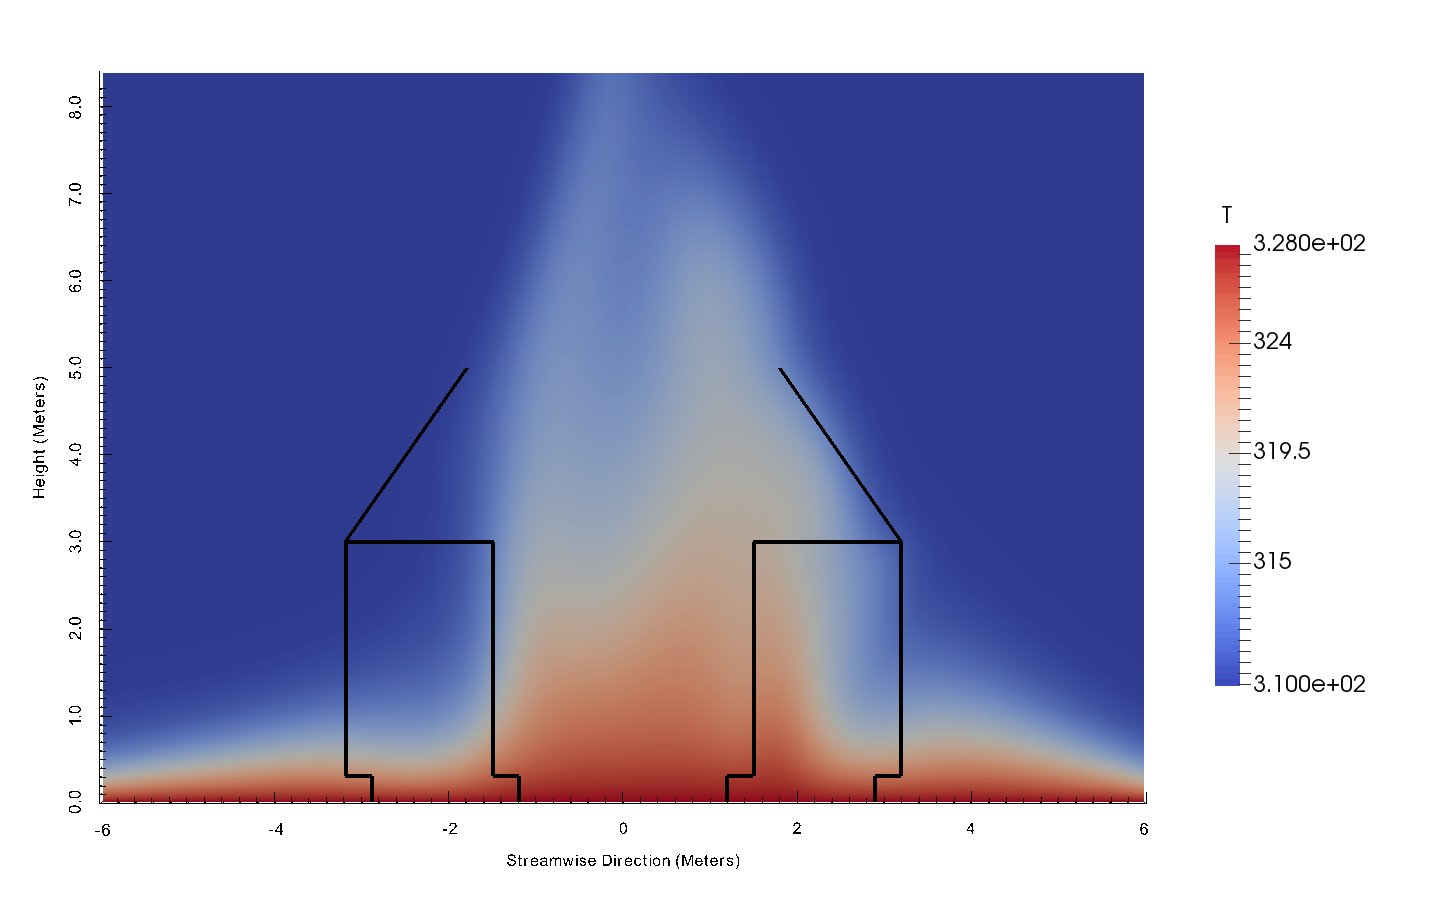
\includegraphics[width=.85\linewidth]{figs/wind_t_vertical}
  \caption{Temperature}
  \label{fig:t-wind-vert}
 \end{subfigure}%
 \begin{subfigure}{.5\textwidth}
  \centering
  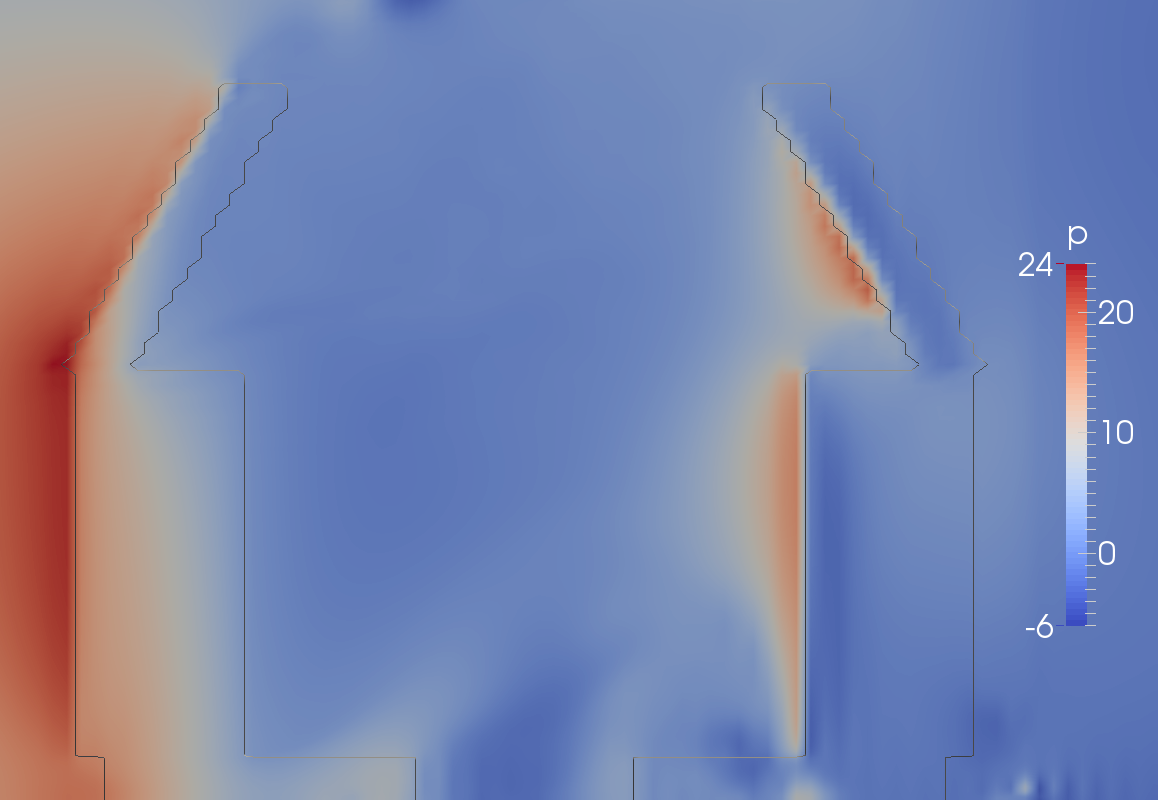
\includegraphics[width=.75\linewidth]{figs/wind_p_vertical}
  \caption{Pressure}
  \label{fig:p-wind-vert}
 \end{subfigure}%

 \caption{Vertical slices for the wind cases.}
 \label{fig:wind-ver}
\end{figure}

The vertical slices are shown in figure \ref{fig:wind-ver}. In this
case, the lower tier of vanes are where the majority of flow is 
entering the center of the apparatus, while the second tier of vanes are
blocking the ambient wind and providing protection to the vortex column. 

The thermal plume is significantly less
visible than in the thermal-only cases. While the
thermal-plume is necessarily weaker relative to the wind, some of this
is also due to the plume no longer being directly centered in the
flow. The plume is more visible using isocountors to render a
three-dimensional surface. 
To visualize the difference between the vertically varying ambient temperature
and the warmer thermal plume, we use the potential temperature, defined
as, 
\begin{equation}
  \tau(x,y,z) = T(x,y,z) -T_{in}(z) 
   \label{eqn:tau}
\end{equation}
where $T_{in}$ is the inflow temperature, described
in section \ref{sec:bc}. In this way the background potential
temperature is nearly zero, and larger values represent deviations from
the base flow temperature. The isocountour of a three Kelvin is 
shown in figure \ref{fig:field_real}. This value was selected as
it was noted as sufficient for formation of a dust devil by
Sinclair\cite{Sinclair1969}. It is clear from the image that a 
strong thermal column does exist even in the $5 m/s$ wind cases. 

%
% tiso
%
  \begin{figure}[!htb]
   \begin{center}
    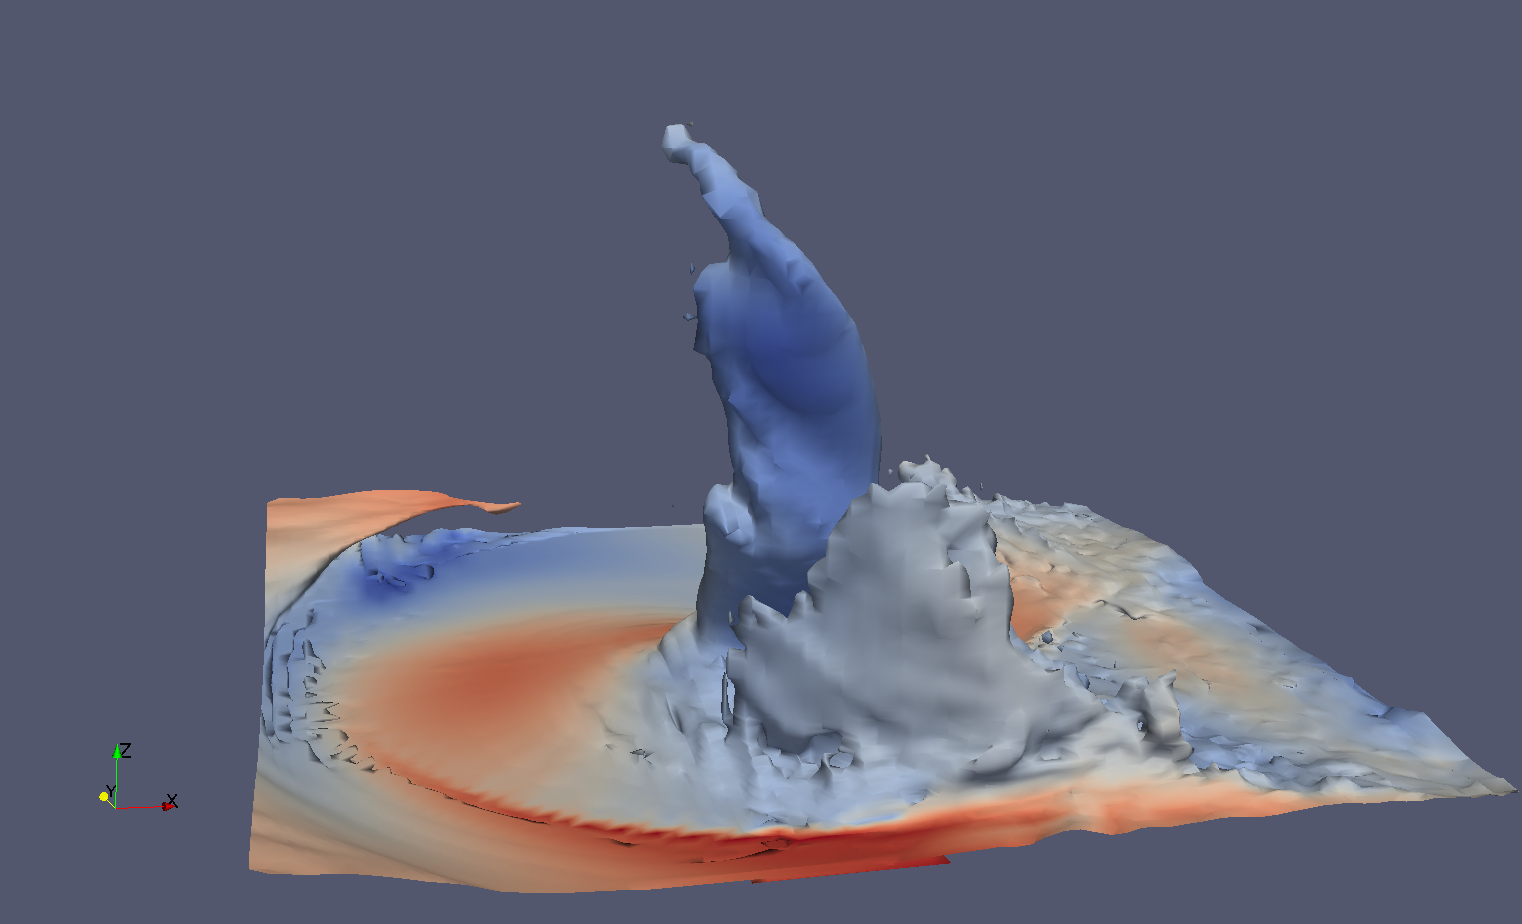
\includegraphics[width = 12 cm]{figs/t_iso}
    \caption{Isocountor of the thermal plume. Here, the isocontour is
    labelled by the potential temperature, $\tau$, as defined in \ref{eqn:tau}.(make this understandible!)}
    \label{fig:field_real}
   \end{center}
  \end{figure}

\subsection{Optimization}

In this section results from a representative optimization
in a thermal-only case are discussed, to demonstrate the optimization 
process employed so far. This is a typical mode of scientific and
engineering inquiry, where a hypothesis regarding system operation is
developed, followed by testing of the hypothesis, and further
iterations.  

This series of simulations are all runs with different system
configurations conducted in a common ambient scenario, that of the
unsteady thermal-only simulations described \todo{add pertinent bcs
here}. 

Our objective is to maximize the energy that can be 
extracted from the synthetic dust devil. As a surrogate to this
quantity, consider the kinetic energy flux through a horizontal plane
near the top of the vanes, where a turbine will ultimately be
placed. This is a surface integral\cite{landau1959fm}

%% \begin{equation}
%%  \dot E = -\oint \rho \textbf{v}(\frac{1}{2}v^2 + e) \cdot d \textbf{f}
%% \end{equation}
%% where $e$ is the internal energy. % and $d\textbf{f}$ the. 
%% For our problem, we consider an incompressible fluid flowing through a
%% flat horizontal region interior to the vanes in the x-y plane, which
%% results in, 

 \begin{equation}
 \dot E = -\frac{\rho }{2} \int V_z (V_{\theta}^2 + V_z^2 ) dA.
 \end{equation}

Using the kinetic energy flux as an objective, the vane geometry has
been optimized. Over approximately  tens of iterations, we have
increased the kinetic energy flux by  a factor of 88 relative to the
baseline. Results of several of these iterations are documented in
figure \ref{fig:opt_plot}. Major adjustments  to design in the the vane
shape and angles were made to obtain this improvement.  Before and after
images shown in \ref{fig:vt-wind-vert}. During this optimization the
qualitative character of the solution changed substantially, changing
from a mild upward flow with little rotation to a strongly organized
vortex with a downward central flow and strong azimuthal velocities.  

\begin{figure}[htb]
 \centering
 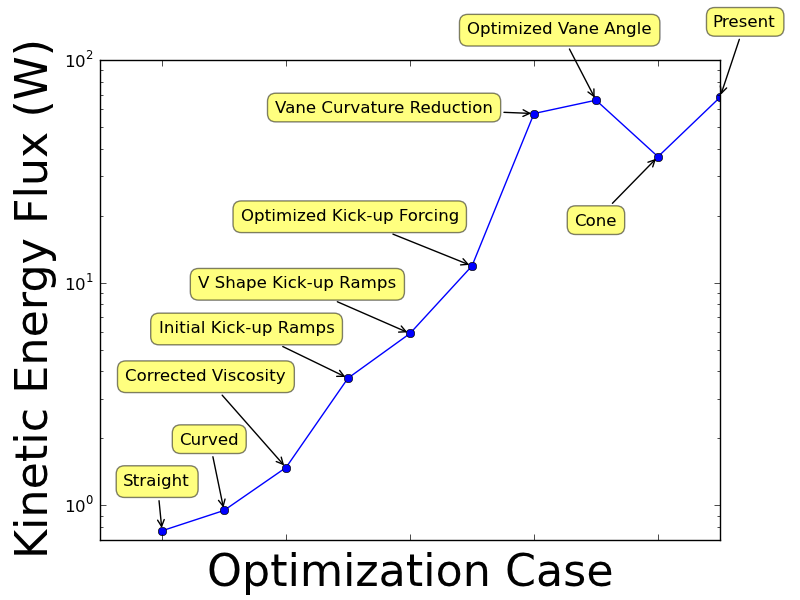
\includegraphics[width=.75\linewidth]{figs/opt_plot}
 \caption{This plot diagrams the improvements to the calculated flux for  
 each iteration of system configuration.}
 \label{fig:opt_plot}
\end{figure}


\begin{figure}[htb!]
 \begin{subfigure}{.5\textwidth}
  \centering
  
\includegraphics[width=.75\linewidth]{figs/before_vanes}
  \caption{Vanes before optimization}
 \end{subfigure}%
 \begin{subfigure}{.5\textwidth}
  \centering
  
\includegraphics[width=.8\linewidth]{figs/after_vanes}
  \caption{Vanes after optimization}
 \end{subfigure}%
 \label{fig:vt-wind-vert}
\end{figure}\todo{need better figure}


%
%
\begin{figure}[htb!]
 \begin{subfigure}{.5\textwidth}
  \centering
  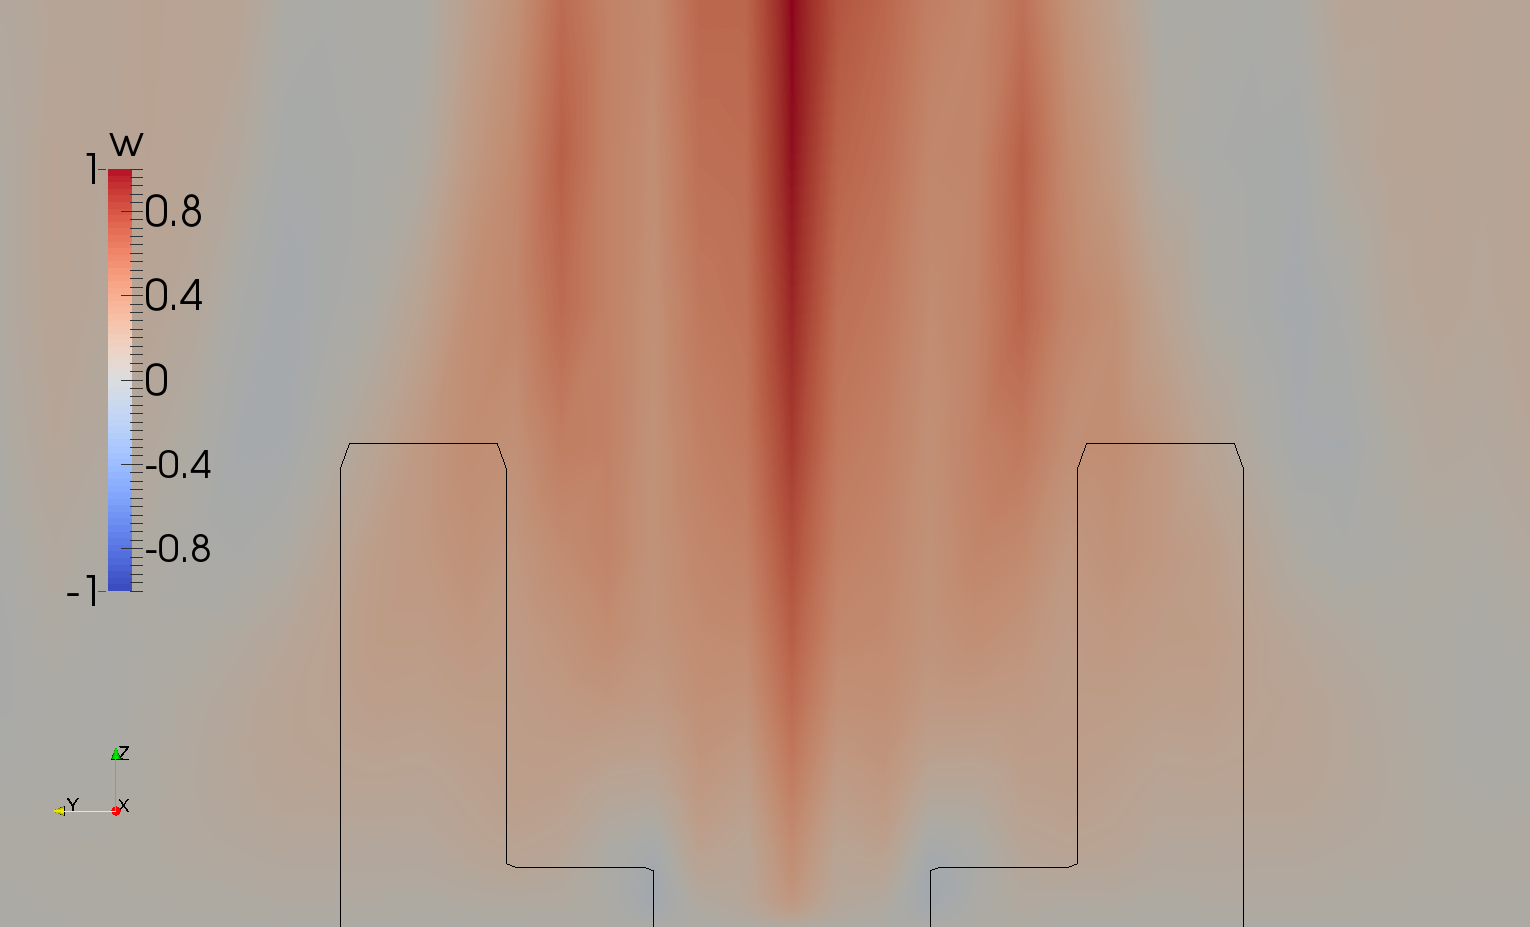
\includegraphics[width=.75\linewidth]{figs/before_opt}
  \caption{Flow before optimization}
 \end{subfigure}%
 \begin{subfigure}{.5\textwidth}
  \centering
  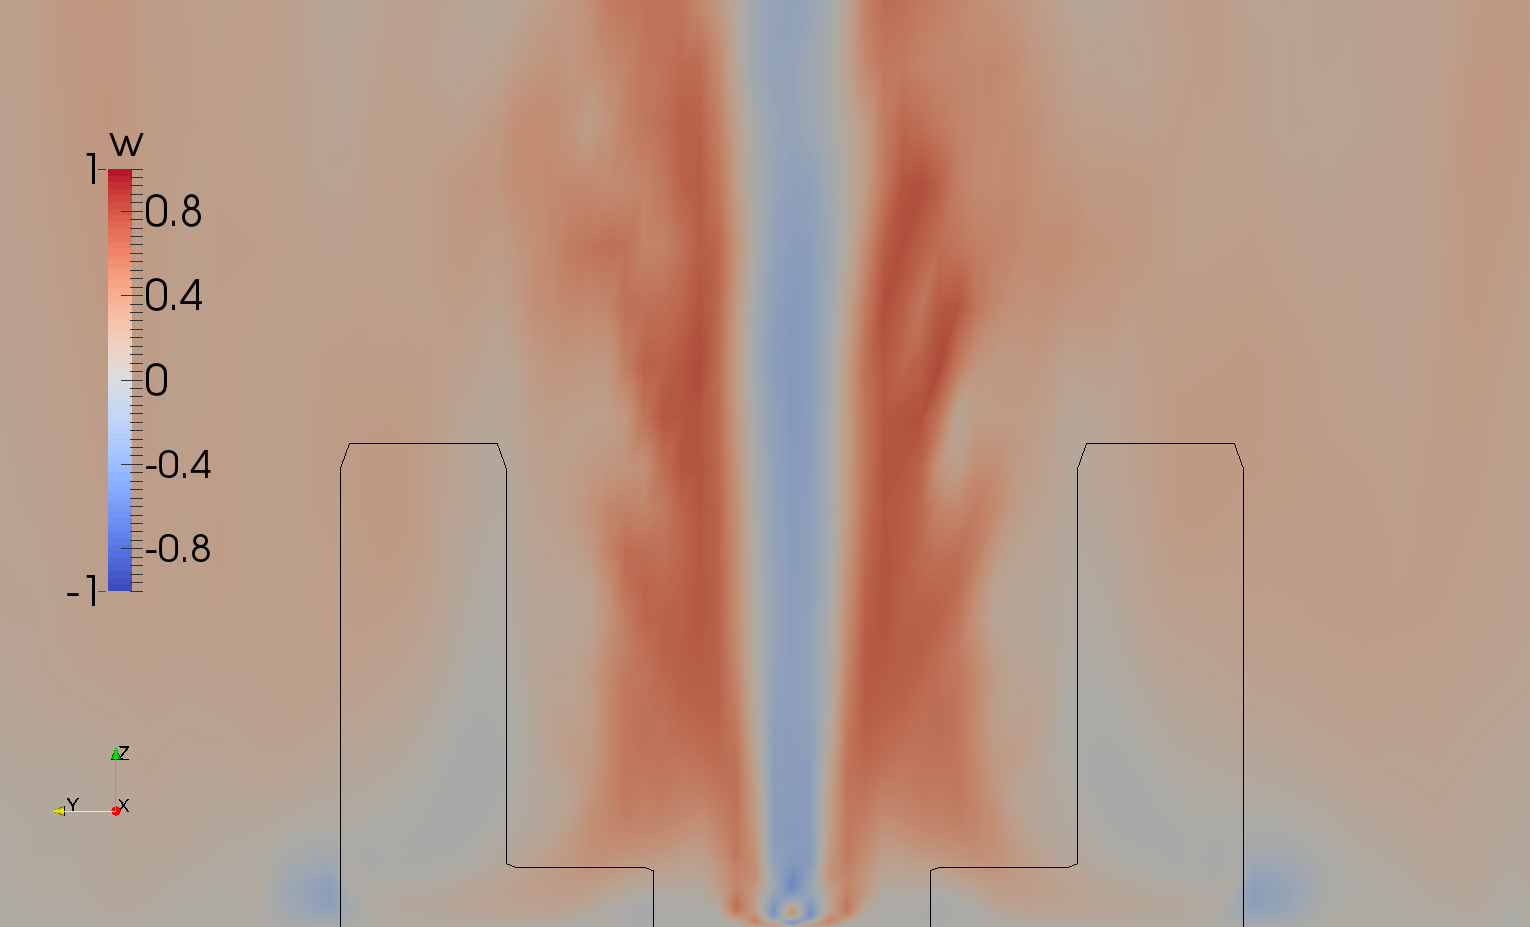
\includegraphics[width=.8\linewidth]{figs/after_opt}
  \caption{Flow after optimization}
 \end{subfigure}%
  \label{fig:opt_flow}
\end{figure}
%
Before and after vertical slices are shown in figure \ref{fig:opt_flow}.


%\section{Summary and Remaining Work}
\section{Proposed Research Campaign}
\label{sec:proposed_work}

\begin{itemize}
\item \st{main event!}
\item ``proposed'' new runs and physical investigation
\item rough time line
\item discuss the program of runs designed to explore a wide configuration space
\item calibrated turbine -- and what else?
\item \st{make clear the objective is to assess feasibility, not to prove it can work}
\item make table of 'state of the art' or novel work expected to have been performed
\item what (fundamental) questions do you want to ask?
      \begin{itemize}
      \item Can we link phenomena to naturally occuring?
      \item By what geometries is the flow intensified, and why
      \end{itemize}
\end{itemize}

The objective of this research project is to provide a definitive
assessment of the  
technological feasibility of the entire synthetic columnar vortex
concept as a means of generating usable energy. In the 
previous sections we have briefed the reader on the present state of the
simulation capability. In doing so, we have discussed the physics that
influence dust devils formation, as well as our particular mathematical
models for the ambient conditions as well as the SoV vanes, cone and
turbine. We summarized the numerical discretizations used, the software
stack and the calibration, verification and validation of these
components. The purpose of these sections was to convince the reader of
two major points. The first point is that an accurate, verified and
validated simulation capability has been developed that can quickly
investigate a wide variety of system and scenario settings at a modest
computational cost. The second point is that we have developed
heuristics that permit optimization of any baseline SoV configuration to
a local maximum of energy production, as measured by kinetic energy flux
through the top of the SoV vanes.  

These two points justify the proposed course of work, which is to
broadly sweep through a large space of possible system configurations
and geometries, and in doing so, discover the globally optimal structure
of the SoV apparatus. Coupled with the scaling analysis presented in
section \ref{sec:physics}, we will then be able to predict the
conditions (if any) under which the SoV apparatus will be
technologically competitive with different methods of energy
generation. In other words, the proposed research is designed to assess
feasibility, and it is not expected that actual experimental validation
will accompany the computational results. Furthermore, it must also be
emphasized that feasibility here is focused on technological capability,
and will not include an economic assessment. In other words, it is
possible that the SoV will produce energy, but the design required to do
is prohibitively expensive, and therefore not economically competitive
with existing technologies. 

%
% outline parameter space, as we see it
%

%
% how many runs are we capable of performing, realistically
%

%
% introduce concept of subdomains
%
We now outline a program of runs designed to explore a wide
configuration space. We begin by noting that we have three 
optimization domains, for the cone, turbine and vanes. Table
\ref{tab:vane} lists the proposed optimization parameters for the
vanes.  

%
% vane optimization
%
\large
\begin{center}
\begin{table}[h]
 \centering
  \begin{tabular}{| l | c | l |}
    \hline
    Parameter & Description & Range \\
    \hline
    $\theta^{\text{t}}_{\text{min}}$ & Starting, minimum angle of the
       top tier & ( 0 - $\theta^{\text{t}}_{\text{max}}$ ) \\
    $\theta^{\text{t}}_{\text{max}}$ & Ending, maximum angle of the top
       tier & ( 0 - 90 ) \\
    $\theta^{\text{b}}_{\text{min}}$ & Starting, minimum angle of the
       bottom tier & ( 0 - $\theta^{\text{b}}_{\text{max}}$ ) \\
    $\theta^{\text{b}}_{\text{max}}$ & Ending, maximum angle of the
       bottom tier & ( 0 - 90 ) \\
   $\gamma$ & Rate of curving & ( 0 - 3 ) \\
   $1 - (r_{\text{min}} / r_{\text{max}})^{\text{t}}$ & Length of the top
       tier vane & ( 0 - 1 ) \\
   $1 - (r_{\text{min}} / r_{\text{max}})^{\text{b}}$ & Length of the bottom
       tier vane & ( 0 - 1 ) \\
   $H^b/H^t$ & Ratio of heights between bottom and top tiers & ( 0 -
	   0.25 ) \\ 
   $D/H$ & Ratio of apparatus diameter and total vane height & ( 0.5 -
	   4.0 ) \\ 
    \hline
  \end{tabular}
  \caption{Vane Optimization Parameters.}
  \label{tab:vane}
\end{table}
\end{center}
\normalsize

explain why 4.0 is plausible

%
% turbine optimization
%
\large
\begin{center}
\begin{table}[h]
 \centering
  \begin{tabular}{| l | c | l |}
    \hline
    Parameter & Description & Range \\
    \hline
    $\theta^{\text{t}}_{\text{min}}$ & Starting, minimum angle of the
       top tier & ( 0 - $\theta^{\text{t}}_{\text{max}}$ ) \\
    $\theta^{\text{t}}_{\text{max}}$ & Ending, maximum angle of the top
       tier & ( 0 - 90 ) \\
    $\theta^{\text{b}}_{\text{min}}$ & Starting, minimum angle of the
       bottom tier & ( 0 - $\theta^{\text{b}}_{\text{max}}$ ) \\
    $\theta^{\text{b}}_{\text{max}}$ & Ending, maximum angle of the
       bottom tier & ( 0 - 90 ) \\

   $\gamma$ & Rate of curving & ( 0 - 3 ) \\
   $r_{\text{min}}$ & 8 & 9 \\
    \hline
  \end{tabular}
  \caption{Turbine Optimization Parameters.}
  \label{tab:turbine}
\end{table}
\end{center}
\normalsize

%
% cone optimization
%
\large
\begin{center}
\begin{table}[h]
 \centering
  \begin{tabular}{| l | c | l |}
    \hline
    Parameter & Description & Range \\
    \hline
    $\theta^{\text{t}}_{\text{min}}$ & Starting, minimum angle of the
       top tier & ( 0 - $\theta^{\text{t}}_{\text{max}}$ ) \\
    $\theta^{\text{t}}_{\text{max}}$ & Ending, maximum angle of the top
       tier & ( 0 - 90 ) \\
    $\theta^{\text{b}}_{\text{min}}$ & Starting, minimum angle of the
       bottom tier & ( 0 - $\theta^{\text{b}}_{\text{max}}$ ) \\
    $\theta^{\text{b}}_{\text{max}}$ & Ending, maximum angle of the
       bottom tier & ( 0 - 90 ) \\
    \hline
  \end{tabular}
  \caption{Cone Optimization Parameters.}
  \label{tab:cone}
\end{table}
\end{center}
\normalsize

shed light on 
the mechanisms by which the apparatus configuration dictates the flow 

%
% can we optimize? DAKOTA
%




In summary, in addition to the preliminary results, several tasks need
to be finished to fulfill the goals of this project:

\begin{itemize}
\item blah
\item yar
\end{itemize}

%
% discussion of risk mitigation 
%
\subsection{Risks and Mitigation}

code ready
expertise ready
plan outlined
ls5 delay?
more compute time
need more runs? this is a serious concern
do we need a comprehensive metric for success?


\newpage
\appendix
\section{Course list}

\begin{table}[h]
\centering
\doublespacing
\begin{tabular}{llll}
\hline \hline
Course Number & Semester & Course Name & Instructor \\ 
\hline 
ME381P  & 2009 Fall   & Fundamentals of incompressible flow                & Dr. D. Bogard \\
EM397   & 2013 Spring & Stabil/multiscale methods in CFD                   & Dr. T. Hughes \\ 
\hline \hline
\end{tabular} 
\end{table}


\bibliography{ref.bib}
\bibliographystyle{plain}


\end{document}
